\documentclass[10pt,a4paper]{article}
\usepackage[T1]{fontenc}
\usepackage[utf8]{inputenc}
\usepackage{lmodern}
\usepackage[margin=2.0cm]{geometry}
\usepackage{booktabs}
\usepackage{array}
\usepackage{tabularx}
\usepackage{xcolor}
\usepackage{amsmath}
\usepackage{pgfplots}
\usepackage{pgfplotstable}
\usepackage{caption}
\usepackage{enumitem}
\usepackage[colorlinks=true,linkcolor=blue!50!black,urlcolor=blue!50!black]{hyperref}
\pgfplotsset{compat=1.17}
\usepgfplotslibrary{groupplots}
\usetikzlibrary{positioning,arrows.meta,shapes.misc}
\captionsetup{font=small,labelfont=bf}
\setlist{nosep,leftmargin=1.4em}
\setlength{\parindent}{0pt}
\setlength{\emergencystretch}{3em}
\renewcommand{\_}{\textunderscore\hspace{0pt}}
\setlength{\parskip}{0.35em}
\renewcommand{\arraystretch}{1.05}
\usepackage[compact]{titlesec}
\titlespacing*{\section}{0pt}{1.2em}{0.4em}
\titlespacing*{\subsection}{0pt}{0.9em}{0.3em}
\setcounter{tocdepth}{1}
\renewcommand{\floatpagefraction}{0.8}
\renewcommand{\topfraction}{0.9}
\renewcommand{\textfraction}{0.1}

% open items are shown in red and counted in the log
\newcommand{\todo}[1]{\textcolor{red}{\textbf{[TODO: #1]}}}
\newcommand{\file}[1]{\texttt{\small #1}}
\newcommand{\env}[1]{\texttt{#1}}
\newcommand{\sweep}{s\,/\,sweep}

% plot styles (colour-blind safe, also distinguishable by marker)
\definecolor{cA30}{HTML}{1B9E77}
\definecolor{cH100}{HTML}{D95F02}
\definecolor{cMAX}{HTML}{7570B3}
\definecolor{cMI}{HTML}{E7298A}
\definecolor{cCPU}{HTML}{666666}
\pgfplotsset{
  every axis/.append style={
    grid=major, grid style={gray!25}, tick label style={font=\small},
    label style={font=\small}, legend style={font=\scriptsize, fill=white, fill opacity=0.85, text opacity=1, draw=gray!50},
    unbounded coords=jump,
  },
  a30/.style={color=cA30, mark=square*, thick},
  h100/.style={color=cH100, mark=triangle*, thick},
  max/.style={color=cMAX, mark=diamond*, thick},
  mi/.style={color=cMI, mark=*, thick},
  cpu/.style={color=cCPU, mark=x, thick},
  mybars/.style={ybar, bar width=9pt},
}

\title{ALF on GPUs: technical report on the port of the\\ auxiliary-field QMC sweep\\[0.3em]
\large Branch \texttt{gpu-port-unified}, state of 2026-11-13}
\author{[author]}
\date{2026-11-13}

\begin{document}
\maketitle
\tableofcontents

\section{Summary}

This report describes the GPU port of the ALF auxiliary-field quantum Monte Carlo code that lives on the branch \texttt{gpu-port-unified}. It is built from the Markdown notes in \file{docs/gpu/} and from the verification runs of 2026-11-13. Every number comes from one of those notes. The source file is given in a comment next to the number in the \LaTeX{} source. Missing numbers and open items are marked in red as TODO.

\subsection*{What runs on which hardware}

One source tree builds for four targets (\file{README.md}, \file{BUILD.md}). The default build, \texttt{GPU=none}, leaves the CPU code unchanged.

\begin{table}[h]
\centering
\caption{Build targets and the hardware on which they were run.}
\label{tab:targets}
\begin{tabular}{@{}lp{4.6cm}p{3.6cm}p{4.2cm}@{}}
\toprule
\texttt{GPU=} & Hardware used & Compiler & Libraries \\
\midrule
\texttt{none} & any CPU & any ALF compiler & BLAS/LAPACK \\ % README.md
\texttt{nvidia} & A30, H100 & nvfortran 25.7 / 26.9 & cuBLAS, cuSOLVER \\ % README.md
\texttt{intel} & Max 1550 (SuperMUC-NG Phase 2) & ifx, oneAPI 2025.x & oneMKL, SYCL shim \\ % README.md
\texttt{amd} & MI210 & gfortran 14 (amdgcn offload) & hipBLAS, hipSOLVER, HIP kernels \\ % README.md
\bottomrule
\end{tabular}
\end{table}

The port was developed for the Hubbard model with a space-time point defect (time-dependent hopping, $N_{\rm FL}=2$). It runs the finite-temperature sweep, the local updates (standard, delayed and submatrix), the wraps, the stabilisation and the equal-time and time-displaced measurements on the device. Random numbers, the accept/reject decision, bookkeeping and file output stay on the host. MPI with independent chains and parallel parameter sets (\texttt{PARALLEL\_PARAMS}) work. Real parallel tempering, the projector code, Langevin, HMC and MALA, other Hamiltonians and several other features are refused at setup, and the run then uses the CPU path (Section~\ref{sec:ported}).

\subsection*{Headline speeds}

Table~\ref{tab:headline} gives seconds per sweep for the Hubbard defect model with $\beta=L$, $\Delta\tau=0.1$, submatrix update and \texttt{Nwrap} 10. Numbers are from different sessions and different timers. Section~\ref{sec:perf} lists how each was obtained.

\begin{table}[h]
\centering
\caption{Seconds per sweep, one chain, and aggregate throughput of the best measured layout at $L=24$.}
\label{tab:headline}
\begin{tabular}{@{}lrrl@{}}
\toprule
Platform and layout & $L=24$ & $L=32$ & Source \\
\midrule
A30, one chain & 5.25 & 18.2 & \file{TUNING\_DEFECT.md} \\ % TUNING_DEFECT.md
A30, 4 ranks with MPS, per chain & 10.5 & \todo{not measured} & \file{MPI\_GPU.md}, \file{README.md} \\ % README.md
H100, one chain & 3.51 & 9.82 & \file{helma\_h100.md} \\ % helma_h100.md 4.1, 4.2
H100, 8 ranks with MPS, per chain & 6.80 & 34.5 & \file{helma\_h100.md} \\ % helma_h100.md
Max 1550, one chain per tile (V7) & 4.95 & 16.4 & \file{ISSUE\_INTEL\_VS\_A30.md} \\ % ISSUE_INTEL_VS_A30.md sec 2
Max 1550, 4 chains per tile, per chain & 9.3 & \todo{not measured} & \file{ISSUE\_INTEL\_VS\_A30.md} \\ % ISSUE_INTEL_VS_A30.md, p7 NOTES
MI210, one process & 4.41 & 17.5 & \file{amd\_mi210/README.md} \\ % platforms/amd_mi210/README.md
\bottomrule
\end{tabular}
\end{table}

The main points:
\begin{itemize}
\item At $L=24$ all four GPUs are within a factor 1.5 of each other for one chain (3.51 to 5.25~s per sweep). The H100 is the fastest at both sizes. At $L=32$ the H100 is 1.8 times faster than the A30 and the MI210 and Max~1550 are close to the A30 (16.4 to 18.2~s).
\item One chain does not fill a GPU. Several chains per GPU raise the throughput by a factor 2 to 4 but slow every chain down by a factor 2 to 3. On the H100 at $L=24$ eight ranks deliver 1.18 sweeps per second against 0.285 for one rank (Section~\ref{sec:mps}).
\item Against one CPU thread the A30 is 28 times faster at $L=24$ and 9.6 times at $L=16$, and not faster at $L=12$ (1.76 against 1.68~s). A CPU comparison with a full node for the defect model does not exist \todo{CPU node-level number for the defect model}.
\item On Intel, run-time switches of one binary reduced the single-chain time at $L=24$ from 10.6 to 4.96~s per sweep (Section~\ref{sec:intel}). The two last steps, device QR and device \texttt{ZUNMQR}, are not yet released for production.
\item MPS is required whenever several ranks share an NVIDIA GPU. Without it, two ranks on an H100 are 6.5 times slower per chain at $L=24$ (Section~\ref{sec:mps}).
\end{itemize}

\subsection*{State of verification}

The GPU build is compared with a CPU build of the same compiler, same parameters and same seeds. Agreement is at rounding level, about $10^{-13}$ with \texttt{Mz = .F.} and about $10^{-10}$ with \texttt{Mz = .T.} (Section~\ref{sec:verif}). The consolidation of the six vendor branches into one was checked on 2026-11-13:
\begin{itemize}
\item \texttt{GPU=none}: four fixed-seed cases are bitwise identical to the pre-merge tip \texttt{cc473abc}. All tested upstream features are bitwise identical to upstream ALF master \texttt{521ddfca} when \texttt{LOBS\_ST = 1} is set. Two differences from upstream are intended.
\item AMD MI210: bitwise identical to the pre-merge AMD tip \texttt{156a0b01} at $L=6$, 12, 16 and 24; timing unchanged.
\item Intel Max~1550 (ifx 2025.3, JIT and AOT builds): against the same-compiler CPU build the deviation is $2.2\times10^{-15}$ and $1.5\times10^{-14}$ ($L=6$ and 12, \texttt{Mz = .F.}) and $5.5\times10^{-11}$ ($L=6$, \texttt{Mz = .T.}). Against the pre-merge Intel build, Green functions, scalars, acceptance and configurations are bitwise identical. With the V7 switches the $L=6$, \texttt{Mz = .T.} value is $1.36\times10^{-10}$, the same as before the merge, above the tolerance of $10^{-10}$.
\item NVIDIA A30: the code builds with nvfortran 26.9; the GPU runs are \todo{pending} (card occupied). NVIDIA H100 (Helma): \todo{pending}.
\end{itemize}

\subsection*{Open points that affect production}

The Intel steps V4 and V7 wait for a numerics review of the device QR. The $L=6$, \texttt{Mz = .T.} test fails its pre-registered tolerance with V7 ($1.36\times10^{-10}$ against $10^{-10}$). The race test of the device QR cannot detect a race on the \texttt{tau} slot. The staging-buffer setting, worth 33\,\% at $L=24$ on Intel, is not in the production job script of the running set. Section~\ref{sec:limits} lists these and the decisions that belong to the owner.

\section{Method in brief}
\label{sec:method}

\subsection{The sweep}

ALF samples a Hubbard--Stratonovich auxiliary field on a space-time lattice with $N$ sites and $L_{\rm trot}=\beta/\Delta\tau$ time slices. For a fixed field the fermions are integrated out. The weight and all equal-time Green functions follow from products of $N\times N$ matrices (\file{PROFILE.md}, \file{HARD.md}). One \emph{sweep} goes up and then down through all slices. In the GPU documents it includes the measurements (\file{TUNING\_DEFECT.md}).

On each slice the code does the following.
\begin{enumerate}
\item \textbf{Local updates.} For every site it proposes a field change, computes the ratio of weights from the Green function $G$, accepts or rejects, and on acceptance updates $G$ by a rank-one matrix. The rank-one update is memory-bound BLAS-2 work.
\item \textbf{Wrap.} It moves $G$ from slice $\tau$ to $\tau+1$ by multiplying with the hopping matrix and the interaction factor.
\item \textbf{Stabilisation.} Every \texttt{Nwrap} slices the product of the $B$ matrices is re-factorised with a QR decomposition, and $G$ is rebuilt (\texttt{CGR}). Between these points the products are numerically unstable.
\item \textbf{Measurements.} Equal-time observables are accumulated from $G$ on every slice. Time-displaced observables (\texttt{Ltau = 1}) need an extra pass over $\tau$ with a $2N\times2N$ factorisation (\texttt{CGR2\_2}).
\end{enumerate}

\subsection{Where the time goes on a CPU}

Table~\ref{tab:cpuprofile} is the profile of the upstream CPU code (stack sampling, one rank, one thread; \file{PROFILE.md}). It is for the plain Hubbard model, $U=4$, $\beta=4$, $\Delta\tau=0.1$, not for the defect model.

\begin{table}[h]
\centering
\caption{Share of wall time per group of routines on one CPU core, in percent (\file{PROFILE.md}). Hubbard square lattice, $U=4$, $\beta=4$, \texttt{Ltau = 1}. cb: checkerboard hopping, dense: dense hopping matrix.}
\label{tab:cpuprofile}
\begin{tabular}{@{}p{5.6cm}rrrrrr@{}}
\toprule
 & \multicolumn{3}{c}{cb} & \multicolumn{3}{c}{dense} \\
\cmidrule(lr){2-4}\cmidrule(lr){5-7}
Group & $12^2$ & $20^2$ & $32^2$ & $12^2$ & $20^2$ & $32^2$ \\
\midrule
Stabilisation (CGR, CGR2\_2, decompose) & 47.0 & 55.4 & 42.3 & 32.0 & 32.0 & 26.4 \\ % PROFILE.md aggregates
Local updates (Upgrade2, Op\_Wrap) & 22.5 & 25.3 & 34.9 & 12.8 & 16.2 & 21.0 \\ % PROFILE.md
$B$ products (wraps, propagators, hopping) & 12.1 & 5.6 & 13.3 & 41.6 & 42.4 & 42.0 \\ % PROFILE.md
Measurements & 16.9 & 11.5 & 8.1 & 11.7 & 6.3 & 5.1 \\ % PROFILE.md
\midrule
Rank-one update (\texttt{ZGERU}) alone & 17.2 & 23.5 & 33.3 & 9.7 & 15.2 & 20.1 \\ % PROFILE.md
Wall time per sweep, 1 rank (s) & 0.60 & 8.0 & 193 & 0.80 & 13.7 & 294 \\ % PROFILE.md
\bottomrule
\end{tabular}
\end{table}

Three points follow for the port (\file{PROFILE.md}, \file{BENCHMARKS.md}):
\begin{itemize}
\item Stabilisation is the largest group. Its QR with column pivoting has no good batched GPU equivalent.
\item The share of the rank-one update grows with $N$ (17 to 33\,\% for checkerboard hopping). It is memory-bound, and one GPU launch per accepted flip is slow. This is the case for delayed and submatrix updates.
\item Measurements are not negligible (17\,\% at $N=144$) and are loops with scatter-adds. They have to run on the device, otherwise $G$ must be copied back three times per slice.
\end{itemize}

The measured cost of one sweep on one core of the \texttt{nividia} host (Zen~3, 16-core EPYC 7763 VM) for the same model is 0.60~s at $N=144$ and 193~s at $N=1024$ with checkerboard hopping (\file{BENCHMARKS.md}). The values at $N=1024$ come from profiling runs with other jobs on the node and are indicative only.

\subsection{Delayed and submatrix updates}

A GPU cannot do rank-one updates fast. Kernel benchmarks on the A30 give 12 to 15~$\mu$s for one OpenMP target region and 28 to 34~$\mu$s for a rank-one update with a host decision at $N\le400$ (\file{BENCHMARKS.md}, \file{ADR-001-programming-model.md}). A rank-$k$ update with $k=128$ costs 0.21 to 1.25~$\mu$s per update on the device, 25 to 40 times less than rank one. This motivates two schemes of ALF (\file{DELAYED\_SUBMATRIX.md}):

\begin{description}
\item[Delayed update.] $G=G_0-XY^{T}$ is kept in low-rank form for up to \texttt{N\_delay} accepted flips and flushed with one \texttt{ZGEMM}.
\item[Submatrix update.] Between flushes only the diagonal wrap scalings change $G_0$. The host copies the principal block $G_0(B,B)$ of one block of \texttt{N\_delay} consecutive vertices once and decides all proposals of the block from it. At the block end the device applies the scalings and flushes with two \texttt{ZGEMM} calls.
\end{description}

On the A30 the block mode brought the submatrix scheme on a $20\times20$ lattice (six sweeps) from 49.7~s to 8.7~s. That is 4.9 times faster than the earlier standard run (42.2~s). Acceptance is identical (\file{DELAYED\_SUBMATRIX.md}). At $L=16$ to $32$ it is 2.4 to 5 times faster than the standard update (\file{TUNING\_DEFECT.md}). The block mode replaced about 8 synchronous device operations per site by about 12 per block.

\subsection{Point defect and time-dependent hopping}

The production model is the Hubbard model with a space-time point defect (\file{TIMEDEP\_HOPPING.md}). A hopping element depends on the time slice through a function $g_t$. The element is applied as $A(g)=U\exp(gE)U^\dagger$ and is skipped when $|g|^2$ is below a threshold. For the point defect the pin is at one slice, $g_t(1)=-1$ ($\tau=0$), after the merge of 2026-11-09. The static hopping is a dense $N\times N$ matrix. The \texttt{Checkerboard} flag is ignored when \texttt{ham\_h0} $\neq0$.

Two consequences matter for the GPU. First, a time-dependent element has one nonzero eigenvalue in the defect case, so it is stored on its support (one site) instead of as a dense matrix. Without this, a set of matrices at $L=32$ needs more than 2~GB. Second, the down sweep measures all slices, including $\tau=0$, and \texttt{SpinZ\_localtau} has $L_{\rm trot}+1-2T_{\rm htrot}$ columns ($\tau=0$ to $\beta$). The default \texttt{LOBS\_ST} is 0; upstream ALF measures $2L_{\rm trot}-1$ times per sweep and the unified branch measures $2L_{\rm trot}$ times (Section~\ref{sec:verif}).

\section{Design}
\label{sec:design}

The design decisions are in two architecture decision records, accepted on 2026-10-27 after the kernel benchmarks of Phase~1 (\file{ADR-001-programming-model.md}, \file{ADR-002-alf-la-and-data-model.md}).

\subsection{Programming model}

ALF is Fortran with class-based Hamiltonians. One source tree has to run with nvfortran, ifx and gfortran, and \texttt{GPU=none} has to stay upstream ALF. The decision (ADR-001) is:

\begin{itemize}
\item \textbf{OpenMP 5.x target offload} with one conservative subset that both nvfortran and ifx accept: \texttt{target enter/exit data}, \texttt{target update}, \texttt{target teams distribute} \texttt{parallel do} on explicit-shape contiguous arrays, and \texttt{use\_device\_addr}. No \texttt{declare mapper}, no unified memory, no polymorphism or allocation in device code.
\item \textbf{Vendor libraries behind one layer, \texttt{alf\_la}.} Large matrix work (\texttt{GEMM}, QR, LU, \texttt{TRSM}) goes to cuBLAS/cuSOLVER, oneMKL or hipBLAS/hipSOLVER. Nothing outside \texttt{alf\_la} knows the backend.
\item \textbf{Selection at configure time}: \texttt{GPU=none|nvidia|intel|amd}.
\item \textbf{Same trajectory as the CPU.} The update is organised as propose, ratio, decide, apply or defer, flush. The decision is made on the host with the same random-number order, so that a GPU run follows the CPU run flip by flip for the same compiler and seeds.
\end{itemize}

OpenACC, CUDA Fortran, \texttt{do concurrent} offload and a SYCL or Kokkos rewrite were considered and not adopted (ADR-001). The only measured difference between OpenMP and OpenACC on the A30 is the asynchronous launch: about 10~$\mu$s for OpenMP \texttt{nowait} and 2.6~$\mu$s for OpenACC \texttt{async} (\file{BENCHMARKS.md}). With a device-side decision per site OpenACC gives 6.5 to 8.8~$\mu$s per site against 15 to 18~$\mu$s for the host decision at $N\le400$. The lever turned out to be algorithmic (delayed and submatrix updates), which removes launches in either model.

The kernel benchmarks (\file{BENCHMARKS.md}) divide the work in two parts. Bulk work, such as stabilisation, dense products and fused element-wise wraps, is 5 to 40 times faster than one core at $N\ge400$. Per-site work is launch-bound: an OpenMP target region costs 12 to 15~$\mu$s, a cuBLAS call 5~$\mu$s and a scalar device-host-device round trip 16 to 23~$\mu$s.

\subsection{Layers}

\begin{figure}[h]
\centering
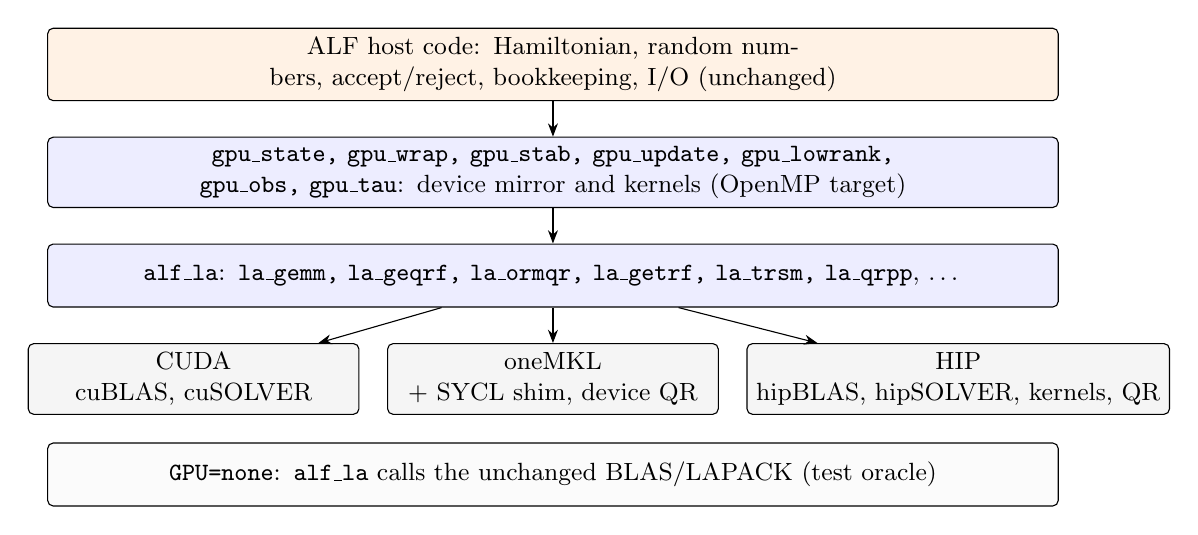
\begin{tikzpicture}[
  box/.style={draw, rounded corners=2pt, minimum height=0.8cm, align=center, font=\small, fill=gray!8},
  dev/.style={box, fill=blue!7},
  host/.style={box, fill=orange!10},
  node distance=0.45cm and 0.35cm]
\node[host, text width=12.6cm] (alf) {ALF host code: Hamiltonian, random numbers, accept/reject, bookkeeping, I/O (unchanged)};
\node[dev, text width=12.6cm, below=of alf] (gpu) {\texttt{gpu\_state, gpu\_wrap, gpu\_stab, gpu\_update, gpu\_lowrank, gpu\_obs, gpu\_tau}: device mirror and kernels (OpenMP target)};
\node[dev, text width=12.6cm, below=of gpu] (la) {\texttt{alf\_la}: \texttt{la\_gemm, la\_geqrf, la\_ormqr, la\_getrf, la\_trsm, la\_qrpp}, \dots};
\node[box, below=of la, minimum width=4.2cm] (mkl) {oneMKL\\+ SYCL shim, device QR};
\node[box, left=of mkl, minimum width=4.2cm] (cu) {CUDA\\cuBLAS, cuSOLVER};
\node[box, right=of mkl, minimum width=4.2cm] (hip) {HIP\\hipBLAS, hipSOLVER, kernels, QR};
\node[box, below=0.35cm of mkl, text width=12.6cm, fill=gray!3] (host2) {\texttt{GPU=none}: \texttt{alf\_la} calls the unchanged BLAS/LAPACK (test oracle)};
\draw[-{Stealth}] (alf) -- (gpu); \draw[-{Stealth}] (gpu) -- (la);
\draw[-{Stealth}] (la) -- (cu); \draw[-{Stealth}] (la) -- (mkl); \draw[-{Stealth}] (la) -- (hip);
\end{tikzpicture}
\caption{Layers of the port. Upstream routines get at most a guarded early branch into the GPU modules (ADR-002).}
\label{fig:layers}
\end{figure}

\subsection{\texttt{alf\_la}}

\texttt{alf\_la\_mod.F90} is one module with plain-array routines in LAPACK argument order: \texttt{la\_gemm}, the real-times-complex variants for dense hopping, strided batched \texttt{GEMM} over flavours, \texttt{la\_geru}, \texttt{la\_geqrf}, \texttt{la\_ungqr}, \texttt{la\_ormqr}, \texttt{la\_getrf}, \texttt{la\_getrs}, \texttt{la\_trsm}, and \texttt{la\_qrpp}, which is a column-norm pre-pivot followed by an unpivoted QR and returns a pivot vector compatible with \texttt{ZGEQP3} (ADR-002). No array descriptors or derived types cross the interface. The arrays are device-resident and \texttt{alf\_la} gets their device addresses through \texttt{use\_device\_addr}.

Library calls must run on the queue that the OpenMP runtime uses for the kernels, otherwise kernels and library calls are not ordered. This was tested and amended in ADR-002:
\begin{itemize}
\item \textbf{CUDA.} A stream created by \texttt{la\_init} is not ordered against nvfortran's target regions. Synchronous regions use the per-thread default stream, so the cuBLAS and cuSOLVER handles are set to the stream returned by \texttt{acc\_get\_cuda\_stream(acc\_async\_sync)}. As a consequence \texttt{nowait} and \texttt{depend} regions are not ordered against library calls. The test \texttt{t\_order} checks this. The build flag \texttt{-DALF\_LA\_SYNC\_ALWAYS} brackets every call with a sync.
\item \textbf{oneMKL.} BLAS goes through \texttt{!\$omp dispatch}. The LAPACK factorisations go through a small SYCL shim on the interop queue of the OpenMP runtime.
\item \textbf{CUDA reproducibility.} cuSOLVER runs in deterministic mode and cuBLAS atomics are off (\file{RUNTIME\_SWITCHES.md}).
\end{itemize}

\subsection{Device-resident data}

\texttt{gpu\_state\_mod.F90} allocates and maps one flat mirror at setup (\texttt{target enter data}) and frees it at the end. Nothing is allocated in loops. Table~\ref{tab:mirror} lists the main arrays (ADR-002).

\begin{table}[h]
\centering
\caption{Main arrays of the device mirror (ADR-002).}
\label{tab:mirror}
\begin{tabular}{@{}lll@{}}
\toprule
Array & Shape & Content \\
\midrule
\texttt{G} & $(N,N,N_{\rm FL})$ & Green function, on the device for the whole run \\ % ADR-002
\texttt{cb\_idx, cb\_exp} & per family & checkerboard bond pairs and $2\times2$ exponentials \\ % ADR-002
\texttt{T\_exp} & $(N,N,N_{\rm FL},4)$ & $e^{\pm T}$, $e^{\pm T/2}$ for dense hopping \\ % ADR-002
\texttt{V\_site, V\_exp} & per \texttt{Op\_V} & sites and exponential table of the diagonal vertices \\ % ADR-002
\texttt{nsigma\_d} & $(N_{\rm op},L_{\rm trot})$ & auxiliary field \\ % ADR-002
\texttt{U, D, V} work, \texttt{udvst\_d} & per stabilisation point & stabilisation stack \\ % ADR-002
\texttt{GT0, G0T, GTT} & $(N,N,N_{\rm FL})$ & time-displaced pass, only for \texttt{Ltau = 1} \\ % ADR-002
\bottomrule
\end{tabular}
\end{table}

The stack dominates memory: peak $\approx(4N_{\rm STM}+40)\cdot16\,N^2$ bytes plus 0.3~GB, with $N_{\rm STM}=L_{\rm trot}/\texttt{Nwrap}$ (\file{TUNING\_DEFECT.md}). The formula gives 19.7~GB at $L=48$, $\beta=48$ and the measurement is 19.6~GB. A card with 24~GB holds $L=48$; for $L=64$ the formula gives 45~GB at $\beta=32$, but $L=64$ cannot be started at present (Section~\ref{sec:limits}).

\subsection{Backends}

\paragraph{CUDA (NVIDIA).} cuBLAS and cuSOLVER through \texttt{bind(C)}. The device of rank $r$ is $r \bmod$ the number of devices. Several ranks per GPU need an MPS daemon (Section~\ref{sec:mps}).

\paragraph{oneMKL and SYCL (Intel).} Beyond the shim, three items were added during the SuperMUC-NG work (\file{ISSUE\_INTEL\_VS\_A30.md}):
\begin{itemize}
\item an \emph{async block path} (\texttt{libalfsb.so}): the block kernels of the submatrix update are submitted on the OpenMP interop in-order queue without a wait (4.3~$\mu$s per operation against 12.3~$\mu$s synchronous);
\item an own \emph{device Householder QR} (\texttt{libalfdevqr.so}, loaded with \texttt{dlopen}) that replaces the hybrid host-device \texttt{geqrf} of oneMKL, in two versions, plus a device \texttt{ZUNMQR};
\item explicit-shape dummy arguments and a fused kernel in the submatrix update, which cut first-private arrays from 168\,800 to 28\,544 per sweep.
\end{itemize}

\paragraph{HIP (AMD).} The AMD build uses gfortran~14 with amdgcn offload. Its libgomp runtime has a high launch cost (\file{amd\_mi210/README.md}). The AMD backend therefore replaces the small OpenMP kernels by HIP kernels (copies, block gather and scale, flush gather, scatter, correlations, scalar and local observables, stabilisation helpers) and adds its own blocked Householder QR and Q-apply. A patched libgomp GCN plugin pools kernel arguments and signals, and calls a presync hook so that HIP calls need no \texttt{hipDeviceSynchronize} after each launch.

\subsection{What stays on the host}

Random numbers, the accept/reject decision, field bookkeeping, bin I/O, the Hamiltonian setup and all of ALF outside the GPU path stay on the host. With the submatrix scheme the host decides all proposals of a block from a copy of the principal block of $G_0$ (\file{DELAYED\_SUBMATRIX.md}). Under \texttt{STABLOG} the CGR factorisations run as host \texttt{ZGEQP3} with copies of the matrices, because no GPU-friendly pivoting met the precision criteria (ADR-001). The time-displaced observables with the defect still use the host \texttt{ObserT} and copy four matrices per $\tau$ slice (\file{TIMEDEP\_HOPPING.md}).

\subsection{Activation, fallback and guard}

At setup \texttt{gpu\_supported} checks the Hamiltonian, the vertices and the options. If a check fails, the whole run uses the CPU path and \texttt{info} gives the reason. It never gives a silent wrong answer. A GPU run should show \texttt{GPU path (gpu\_state): ACTIVE} and \texttt{GPU observables: device equal-time measurement ACTIVE} in \texttt{info}. All runs set \texttt{OMP\_TARGET\_OFFLOAD=MANDATORY}, otherwise a failed device initialisation silently runs on the CPU.

A production guard (\file{RUNTIME\_SWITCHES.md}) reads the environment: any \texttt{ALF\_GPU\_*} or \texttt{ALF\_LA\_TEST\_*} variable except \texttt{ALF\_GPU\_DISABLE} and \texttt{ALF\_GPU\_DEBUG} stops a run unless it is declared a debug run. The variables \texttt{ALFSH\_*}, \texttt{ALF\_HIP\_*} and \texttt{ALFDEVQR\_*} are outside the guard and have to be checked by hand.

\subsection{Compiler problems met}

\begin{table}[h]
\centering
\caption{Compiler and runtime problems that shaped the code or the build.}
\label{tab:compilers}
\small
\begin{tabularx}{\textwidth}{@{}lX@{}}
\toprule
Toolchain & Problem and handling \\
\midrule
nvfortran 26.9 & \texttt{blk\_end} is mis-compiled at \texttt{-O2} and above (wrong $G$ after the first stabilisation). It is pinned to \texttt{-O1} with \texttt{!pgi\$r opt=1}. The cause is not understood (\file{DELAYED\_SUBMATRIX.md}). \\ % DELAYED_SUBMATRIX.md
nvhpc 24.11 & The GPU build compiles but the $L=8$ run aborts with \texttt{la\_qrpp: NaN or Inf}. The CPU run of the same compiler is fine. Not used (\file{helma\_h100.md}). \\ % helma_h100.md
nvhpc 25.7 & Needs \texttt{-gpu=cc90,cuda12.9}; without it the default CUDA 13 device compile fails (\file{helma\_h100.md}). \\ % helma_h100.md
ifx $\le$ 2025.3 & \texttt{omp\_get\_interop\_int/ptr} are missing in \texttt{omp\_lib}, so \texttt{alf\_la\_mod.F90} declares them with \texttt{bind(C)} (\file{intel\_pvc\_supermuc\_ng2.md}). \\ % platforms/intel_pvc_supermuc_ng2.md
oneAPI 2025.3 & Compiles, but the OpenMP-to-SYCL interop crashes at run time with the Level Zero V2 adapter. 2025.1 works and is used (\file{intel\_pvc\_supermuc\_ng2.md}). \\ % intel_pvc_supermuc_ng2.md
ifx (OpenMP tasks) & \texttt{nowait}/\texttt{depend} target tasks run undeferred; no gain (gate A: 97 to 103\,\% of the baseline time) (\file{ISSUE\_INTEL\_VS\_A30.md}). \\ % ISSUE_INTEL_VS_A30.md sec 4
gfortran 14 (amdgcn) & Launch cost of the libgomp GCN plugin is high: 253~$\mu$s for an empty target region, 37~$\mu$s with the patched plugin (\file{amd\_mi210/README.md}). \\ % platforms/amd_mi210/README.md
\bottomrule
\end{tabularx}
\end{table}

\subsection{Source layout}

The device code is in \texttt{Prog/gpu\_*\_mod.F90} (state, wrap, stabilisation, update, low-rank blocks, equal-time and time-displaced observables). The backends are in \texttt{Libraries/Modules/}: \texttt{alf\_la\_mod.F90} (interface and CUDA/oneMKL/host code), \texttt{alf\_la\_sycl\_*} (Intel shim, async block path, device QR) and \texttt{alf\_la\_hip\_mod.F90}, \texttt{alf\_hipk\_mod.F90}, \texttt{alf\_hip\_*.cpp} (AMD). Unit tests of \texttt{alf\_la} and the acceptance harness are in \texttt{testsuite/alf\_la.tests/} and \texttt{testsuite/gpu\_reference/} (\file{README.md}).

\section{What is ported}
\label{sec:ported}

Table~\ref{tab:features} lists the features per backend. The base is \file{FEATURES.md} (state 2026-11-06). Rows on MPI and parallel parameters are updated from \file{MPI\_GPU.md}, \file{PP\_GPU.md}, \file{helma\_h100.md}, \file{intel\_pvc\_supermuc\_ng2.md} and the SuperMUC session notes, which are newer. \todo{\file{FEATURES.md} is stale: it has the Arc B580 as the Intel GPU, lists MPI and tempering as refused on Intel and has no AMD column. It should be updated; the table here follows the newer notes}

Entries: S = supported and validated, R = refused at setup (the run uses the CPU path), N = not implemented (no GPU code and no check, a CPU-only feature that the model does not use), ? = not documented. The AMD notes do not list feature coverage; the AMD column shows only what the notes state. \todo{AMD feature coverage is not documented; fill the ? entries after a check of \texttt{gpu\_supported} on the HIP build}

\begin{table}[h]
\centering
\caption{Feature coverage of the GPU path. NVIDIA: A30 and H100. Intel: Max 1550 (the first notes were for an Arc B580).}
\label{tab:features}
\small
\begin{tabular}{@{}p{6.1cm}cccc@{}}
\toprule
Feature & CPU & NVIDIA & Intel & AMD \\
\midrule
Finite-$T$ DQMC, Hubbard (predefined) & S & S & S & S \\ % FEATURES.md; AMD: platforms/amd_mi210/README.md (defect production parameters)
Projector ($T=0$) & S & R & R & ? \\ % FEATURES.md
Other Hamiltonians (Plain\_Vanilla, Kondo, tV, Spin\_Peierls, $Z_2$, LRC) & S & R & R & ? \\ % FEATURES.md
HS fields type 1, 2 (diagonal, rank-1) & S & S & S & ? \\ % FEATURES.md
HS fields type 3, 4; non-diagonal or rank $>1$ vertices & S & R & R & ? \\ % FEATURES.md
Local updates, standard & S & S & S & ? \\ % FEATURES.md; Intel measured in p7 NOTES.md sec 5
Delayed and submatrix updates & S & S & S & S \\ % FEATURES.md, DELAYED_SUBMATRIX.md; AMD README submatrix runs
Cross-slice delay (\texttt{Lowrank\_cross\_slice}) & S & R & R & ? \\ % FEATURES.md
Global-in-$\tau$ and space-time moves & S & R & R & ? \\ % FEATURES.md
Langevin, HMC, MALA & S & R & R & ? \\ % FEATURES.md
Parallel tempering (exchange) & S & R & R & ? \\ % FEATURES.md, PP_GPU.md
Parallel parameter sets (\texttt{PARALLEL\_PARAMS}), no exchange & S & S & S & ? \\ % PP_GPU.md, helma_h100.md, intel_pvc_supermuc_ng2.md
MPI, independent chains & S & S & S & ? \\ % MPI_GPU.md, intel_pvc_supermuc_ng2.md
Checkerboard, dense hopping, \texttt{Symm} & S & S & S & ? \\ % FEATURES.md
Time-dependent hopping (point defect) & S & S & S & S \\ % TIMEDEP_HOPPING.md; AMD README
Time-dependent couplings of \texttt{Op\_V} & S & R & R & ? \\ % FEATURES.md
Flavour symmetry reconstruction & S & R & R & ? \\ % FEATURES.md
Stabilisation default (pre-pivoted QR) & S & S & S & S \\ % ADR-001
Stabilisation \texttt{LOG} (host QR with pivoting) & S & S & S & ? \\ % ADR-001, FEATURES.md
\texttt{STAB1/2/3}, \texttt{QRREF}, \texttt{Propose\_S0} & S & R & R & ? \\ % FEATURES.md
Equal-time observables (Hubbard) & S & S & S & S \\ % FEATURES.md
Time-displaced observables (\texttt{Ltau = 1}) & S & S & S & ? \\ % FEATURES.md, TIMEDEP_HOPPING.md
Custom observables, entanglement & S & N & N & N \\ % FEATURES.md
HDF5 output (host side) & S & S & S & ? \\ % MPI_GPU.md (L16 run), helma_h100.md
\bottomrule
\end{tabular}
\end{table}

\subsection*{Remarks on the table}

\begin{itemize}
\item The GPU path is taken only if every check passes. Otherwise the whole run uses the CPU path, and \texttt{info} states the reason (\file{FEATURES.md}).
\item The time-displaced pass for the defect runs its propagation on the device, but the $\tau$ observables with the defect still use the host \texttt{ObserT} (\file{TIMEDEP\_HOPPING.md}). \texttt{Ltau = 0} is recommended; \texttt{Ltau = 1} works but is slower (\file{TUNING\_DEFECT.md}).
\item Time-dependent hopping elements are accepted only if they follow all static elements in \texttt{Op\_T(:,nf)}. Otherwise the run is refused with a reason (\file{TIMEDEP\_HOPPING.md}).
\item Tempering is refused only as real tempering. Since the change of \texttt{gpu\_state\_mod.F90} (\file{PP\_GPU.md}), builds with \texttt{PARALLEL\_PARAMS} are accepted and \texttt{Exchange\_Step} is skipped in \texttt{main.F90}.
\item On one Max~1550 tile the standard and delayed schemes were also timed at $L=24$: 18.32 and 19.66~s per sweep against 5.01~s for the submatrix scheme (\file{ISSUE\_INTEL\_VS\_A30.md}, \file{p7/NOTES.md}).
\end{itemize}

\subsection*{Not implemented, by group (\file{NOT\_IMPLEMENTED.md})}

\begin{description}
\item[Model and feature coverage.] Rank $>1$ and non-diagonal vertices (would open tV, Kondo, Spin\_Peierls); flavour-symmetry reconstruction (Plain\_Vanilla, Spin\_Peierls); device observables for other models, entanglement and custom observables; HS fields of type 3 and 4; global moves; \texttt{Propose\_S0}; time-dependent couplings of \texttt{Op\_V}; \texttt{STAB1/2/3} and \texttt{QRREF}; cross-slice delay; parallel tempering; projector; Langevin and HMC.
\item[Performance at small and medium $N$.] Device-side accept decision, start-up cost, per-bin output, remaining launch overhead.
\item[Performance at large $N$.] Sparse \texttt{Symm}, a memory footprint of about $1650\,N^2$ bytes, block structure of the $\tau$ pass, Cholesky-QR variants.
\end{description}

\subsection*{Size limits}

At $\beta=5$ a $62\times62$ lattice fits an A30 (23\,967~MiB) and $63\times63$ does not (\file{DELAYED\_SUBMATRIX.md}). In the defect setting with $\beta=L$ the peak memory is 3077~MiB at $L=32$ and 19\,647~MiB at $L=48$ (\file{TUNING\_DEFECT.md}). The H100 uses 3584~MiB per rank at $L=32$ (\file{helma\_h100.md}).

\section{Verification}
\label{sec:verif}

\subsection{Method}

\paragraph{Same-compiler CPU reference.} A GPU build is compared with a CPU build (\texttt{GPU=none}) made by the same compiler, with the same parameters and the same seeds. The CPU reference must come from the same compiler because the random-number stream of the GNU build differs from that of nvfortran, so trajectories from different compilers are not comparable (\file{TIMEDEP\_HOPPING.md}). With the same seeds and the host decision of ADR-001 the GPU trajectory follows the CPU trajectory flip by flip until rounding differences accumulate. The driver is \texttt{scripts/defect/run\_cmp.py} (\file{VERIFICATION.md}, \file{README.md}).

\paragraph{Deviation measure.} For each output file the deviation is $\max|A-B|/\max|A|$ over the file. Acceptance rates and final configurations have to be identical.

\paragraph{Tolerances.} About $10^{-13}$ for \texttt{Mz = .F.} and about $10^{-10}$ for \texttt{Mz = .T.} (\file{README.md}). The Intel session used the same two values; the SuperMUC first session used $10^{-8}$ as the criterion (\file{intel\_pvc\_supermuc\_ng2.md}). The \texttt{Mz = .T.} deviations are the intrinsic accuracy of $G$ and not a code difference: the same code gives $10^{-14}$ with \texttt{Mz = .F.} (\file{TIMEDEP\_HOPPING.md}). Production runs additionally monitor \texttt{Precision Green}; the requirement in the Helma benchmarks is below $10^{-8}$ (\file{helma\_h100.md}).

\paragraph{Test standard} (\file{VERIFICATION.md}, from 2026-10-29). The main rules are:
\begin{itemize}
\item Acceptance runs use binaries built from \texttt{git archive} of a frozen candidate. The committed tree equals the accepted tree except for \texttt{docs/**}.
\item Every run writes a provenance record (candidate hash, binary hash, compiler, environment, parameter and seed hashes, output hashes). Debug and fault variables are refused unless the acceptance file declares a test run. GPU runs have to show the \texttt{ACTIVE} lines.
\item Each ticket has a pre-registered acceptance file with gates, thresholds, seeds and positive controls. Changing it needs the owner's dated approval and fresh seeds.
\item Verdicts are computed by a script. NaN, missing files and inactive GPU paths give \texttt{INPUT\_ERROR}, never a pass.
\item Every gate has a positive control that must fail, for example a scaled tau dataset, \texttt{ALF\_GPU\_NS=0} or a planted $10^{-12}$ perturbation. Statistical gates carry a null control (CPU against CPU).
\item Tiers: T0 (every iteration), T1 (implementer, frozen candidate, about 90~min GPU time) and T2 (manager, fresh seeds, about 120~min, plus an independent verifier).
\end{itemize}

\paragraph{Determinism.} Where bit identity holds (same binary run twice, same commit rebuilt with the same toolchain), it is demanded. On 2026-10-29 the \texttt{LOG} path on the A30 was bitwise reproducible, the default path was not (20 of 38 datasets differed, first in \texttt{Den\_eq/back} at about $10^{-12}$ relative). MPS and CPU jobs alongside did not change results (\file{VERIFICATION.md}). \todo{state of ticket 212 (reproducibility of the default path); the notes do not say whether it is closed}

\subsection{Earlier results against the same-compiler CPU reference}

Table~\ref{tab:earlier} collects the same-seed results from the platform sessions before the merge.

\begin{table}[h]
\centering
\caption{Worst relative deviation, GPU against the same-compiler CPU build, same seeds. Acceptance identical in all rows.}
\label{tab:earlier}
\small
\begin{tabularx}{\textwidth}{@{}p{2.6cm}p{5.2cm}Xp{2.9cm}@{}}
\toprule
Platform & Case & Deviation & Source \\
\midrule
A30, nvfortran 26.9 & $U=0$, $L=4$ and $L=8$, all files & $3.0\times10^{-14}$, $8.5\times10^{-14}$ & \file{TIMEDEP\_HOPPING.md} \\ % TIMEDEP_HOPPING.md sec 5
A30 & $L=4$, \texttt{Mz = .F.}, standard, delayed, submatrix & $1.7$, $1.5$, $2.2\times10^{-15}$ & \file{TIMEDEP\_HOPPING.md} \\ % TIMEDEP_HOPPING.md
A30 & $L=8$, \texttt{Mz = .F.}, three schemes & $8.4\times10^{-15}$ & \file{TIMEDEP\_HOPPING.md} \\ % TIMEDEP_HOPPING.md
A30 & $L=8$, \texttt{Mz = .T.}, three schemes & $5.1\times10^{-10}$ (largest in \texttt{SpinZ\_localtau}) & \file{TIMEDEP\_HOPPING.md} \\ % TIMEDEP_HOPPING.md
A30 & $L=32$, $\beta=4$, 1 sweep, \texttt{Mz = .F.} standard, delayed & $6.0\times10^{-15}$, $1.4\times10^{-14}$ & \file{TIMEDEP\_HOPPING.md} \\ % TIMEDEP_HOPPING.md
A30 & one MPI rank against non-MPI, $L=16$ & $10^{-12}$ level (\texttt{Ener\_scal} $7\times10^{-12}$, \texttt{SpinZ\_localtau} $1.4\times10^{-12}$) & \file{MPI\_GPU.md} \\ % MPI_GPU.md
H100, nvhpc 25.7 & $L=8$, \texttt{Mz = .F.}, $N_{\rm delay}$ 64 & $5.2\times10^{-13}$ & \file{helma\_h100.md} \\ % helma_h100.md sec 3
Max 1550, ifx & \texttt{Mz = .F.}, $L=6$ to 12, $N_{\rm delay}$ 8 to 128 & $3.0\times10^{-15}$ to $2.7\times10^{-14}$ & \file{intel\_pvc\_supermuc\_ng2.md} \\ % intel_pvc_supermuc_ng2.md
Max 1550, ifx & \texttt{Mz = .T.}, $L=6$ ($L=12$, $N_{\rm delay}$ 128) & $2.5\times10^{-11}$ ($3.4\times10^{-9}$) & \file{intel\_pvc\_supermuc\_ng2.md} \\ % intel_pvc_supermuc_ng2.md
Max 1550, V4 & \texttt{Mz = .F.} $L=6$, $L=12$; \texttt{Mz = .T.} & $2.2\times10^{-15}$, $1.6\times10^{-14}$; $6.0\times10^{-11}$ & \file{ISSUE\_INTEL\_VS\_A30.md} \\ % ISSUE_INTEL_VS_A30.md sec 5
Max 1550, V7 & \texttt{Mz = .F.} $L=6$, $L=12$; \texttt{Mz = .T.} $L=6$ & $2.3\times10^{-15}$, $1.6\times10^{-14}$; $1.36\times10^{-10}$ (fails $10^{-10}$) & \file{ISSUE\_INTEL\_VS\_A30.md} \\ % ISSUE_INTEL_VS_A30.md sec 7
\bottomrule
\end{tabularx}
\end{table}

For V7 the criterion is noise-limited. oneMKL itself fails the $L=6$, \texttt{Mz = .T.} tolerance for 2 of 5 seed sets ($1.13\times10^{-10}$ and $1.84\times10^{-10}$). A new pre-registered rule needs the owner's approval (\file{ISSUE\_INTEL\_VS\_A30.md}).

\paragraph{Physics and statistics.} Delayed and submatrix reproduce the standard update bin by bin on the A30 and on the B580 and agree with exact diagonalisation of a four-site chain within one standard deviation (\file{DELAYED\_SUBMATRIX.md}). The upstream \texttt{test\_vs\_ed} Hubbard chain passes with GNU, ifx and nvfortran (deviations of 0.64, 1.48 and 1.52 standard deviations, \file{BASELINE.md}).

\paragraph{Precision of $G$ at production sizes.} \texttt{Precision Green} (mean / max) at $L=24$, 28, 32 on the Max~1550 is $1.7\times10^{-14}/1.2\times10^{-11}$, $4.6\times10^{-14}/1.1\times10^{-10}$ and $1.4\times10^{-13}/5.3\times10^{-10}$ (\file{intel\_pvc\_supermuc\_ng2.md}). On the H100 at $L=32$ the maximum is $1.4\times10^{-10}$ to $7.2\times10^{-10}$ in all configurations (\file{helma\_h100.md}).

\subsection{Verification of the consolidated branch, 2026-11-13}
\label{sec:verif1113}

\texttt{gpu-port-unified} merges six vendor lines (\file{CONSOLIDATION.md}). The checks below test that the merge changed nothing it should not have changed. They were run on 2026-11-13. Entries that were not finished when this report was written are marked \todo{pending}. Source of the Intel and AMD rows: the verification table of \file{CONSOLIDATION.md}.

\begin{table}[h]
\centering
\caption{Checks of the consolidated branch. Source of all entries: verification runs of 2026-11-13.}
\label{tab:verif1113}
\small
\begin{tabularx}{\textwidth}{@{}p{3.1cm}p{4.2cm}Xl@{}}
\toprule
Platform, build & Comparison & Result & Status \\
\midrule
macOS, gfortran 16, \texttt{GPU=none} & 4 fixed-seed cases ($L=4$/6, \texttt{Mz} T/F, delayed/submatrix) against the pre-merge tip \texttt{cc473abc} & bitwise identical & done \\ % verification 2026-11-13
macOS, gfortran, \texttt{GPU=none}, $L=4$ & upstream ALF master \texttt{521ddfca}, \texttt{LOBS\_ST = 1} set explicitly & bitwise identical for all tested upstream features (list below) & done \\ % verification 2026-11-13
\texttt{GPU=none}, gfortran & delayed and submatrix against the standard update & agree to $10^{-12}$ with identical trajectories & done \\ % verification 2026-11-13
\texttt{GPU=none}, gfortran & \texttt{SpinZ\_localtau} against an exact $U=0$ calculation & agrees to $4.7\times10^{-14}$ & done \\ % verification 2026-11-13
AMD MI210, \texttt{GPU=amd}, gfortran 14 GCN + HIP & unified against pre-merge tip \texttt{156a0b01}, $L=6$, 12, 16, 24; default, \texttt{ALF\_HIP\_ASYNC=0}, \texttt{ALF\_HIP\_QR=0} & bitwise identical in all cases & done \\ % verification 2026-11-13
AMD MI210 & GPU against same-compiler CPU & $1.15\times10^{-14}$ ($L=6$), $5.0\times10^{-14}$ ($L=12$) & done \\ % verification 2026-11-13
AMD MI210 & timing & unchanged, about 4.5~s per sweep at $L=24$ & done \\ % verification 2026-11-13
NVIDIA A30, nvfortran 26.9 & build of GPU and CPU reference & builds & done \\ % verification 2026-11-13
NVIDIA A30 & GPU runs & \todo{pending} (card occupied by a production run) & pending \\ % verification 2026-11-13
NVIDIA H100 (Helma) & GPU runs & \todo{pending} & pending \\ % verification 2026-11-13
Intel Max 1550 (SuperMUC-NG Phase 2), ifx 2025.3, JIT and AOT & GPU against same-compiler CPU, default switches & $2.2\times10^{-15}$ ($L=6$, \texttt{Mz = .F.}), $1.5\times10^{-14}$ ($L=12$, \texttt{Mz = .F.}), $5.5\times10^{-11}$ ($L=6$, \texttt{Mz = .T.}) & done \\ % CONSOLIDATION.md
Intel Max 1550, V7 switches & GPU against same-compiler CPU & $2.3\times10^{-15}$, $1.6\times10^{-14}$, $1.36\times10^{-10}$ ($L=6$, \texttt{Mz = .T.}; same value as before the merge, tolerance $10^{-10}$, fails) & done, one failure \\ % CONSOLIDATION.md
Intel Max 1550 & unified against pre-merge Intel build (p5) & Green functions, scalars, acceptance and configurations bitwise identical; \texttt{Den\_eq}, \texttt{SpinT\_eq}, \texttt{SpinZ\_eq} differ by at most $3.3\times10^{-16}$ (expected, \texttt{acc0} parallel reduction from pp-opt) & done \\ % CONSOLIDATION.md
Intel Max 1550, $L=24$, one chain, V7 & timing, before and after the merge & 4.92 to 4.98~s per sweep before, 4.42 to 4.48~s after; observables 1.18 to 0.74~s per sweep; updates 1.43, stabilisation 0.81, CGR 1.23~s unchanged & done \\ % CONSOLIDATION.md
\bottomrule
\end{tabularx}
\end{table}

\paragraph{Upstream features tested for bitwise identity} against ALF master \texttt{521ddfca}, with \texttt{GPU=none}, gfortran, $L=4$ and \texttt{LOBS\_ST = 1}: Hubbard with \texttt{Mz} true and false, \texttt{Symm}, checkerboard, \texttt{Ltau} 0 and 1, projector, \texttt{N\_SUN}, continuous fields, Langevin, HMC, MALA, Kondo, tV and Plain Vanilla.

\paragraph{Two intended differences from upstream.}
\begin{enumerate}
\item The default \texttt{LOBS\_ST} is 0. The down sweep then also measures at $\tau=0$, which gives $2L_{\rm trot}$ instead of $2L_{\rm trot}-1$ measurements per sweep. With \texttt{LOBS\_ST = 1} the upstream behaviour is restored.
\item \texttt{ham\_h0} now means the space-time point defect and not upstream's static pinning field.
\end{enumerate}

\paragraph{Limits of these checks.} The \texttt{GPU=none} checks show that the merge did not change the CPU path. They say nothing about the device code, which was checked on the MI210 and on the Max~1550. The two pending NVIDIA rows (A30, H100) have to be run before the consolidated branch can be called verified on NVIDIA. The Intel jobs 560852 to 560860 used about 0.85 node-hours. The CI (\texttt{.github/workflows/tests.yml}) builds and tests the CPU path only (\file{README.md}). The \texttt{acc0} parallel reduction that arrived from the pp-opt line changes the summation order of the \texttt{acc0} terms. On the Max~1550 the effect is at most $3.3\times10^{-16}$ in \texttt{Den\_eq}, \texttt{SpinT\_eq} and \texttt{SpinZ\_eq}, and it cuts the observables phase from 1.18 to 0.74~s per sweep, about 10\,\% of the sweep (\file{CONSOLIDATION.md}).

\section{Performance}
\label{sec:perf}

\subsection{How the numbers were obtained}

The numbers come from different sessions on different machines. Table~\ref{tab:how} states how each was measured. They are comparable to within the differences stated there, not better.

\begin{table}[h]
\centering
\caption{Measurement method per platform. All runs: Hubbard defect model, $N_{\rm FL}=2$, $h_0=1$, \texttt{Mz = .F.}, $\beta=L$, $\Delta\tau=0.1$, \texttt{Nwrap} 10, submatrix, unless stated.}
\label{tab:how}
\small
\begin{tabularx}{\textwidth}{@{}lX@{}}
\toprule
Platform & Method \\
\midrule
A30 (\texttt{nividia}) & nvfortran 26.9, one process, 2 sweeps, timer in the run, excludes the 1 to 2~s mirror set-up (\file{TUNING\_DEFECT.md}). The older multi-rank numbers are CPU time of rank 0 divided by the number of sweeps and include start-up. Whether MPS was active in those runs is not recorded (\file{helma\_h100.md}). \\ % TUNING_DEFECT.md, helma_h100.md 4.1
H100 (Helma) & nvhpc 25.7, 6 sweeps per test (\texttt{NSweep} 2, \texttt{NBin} 3), (finish time $-$ start time)/6 of rank 0. Excludes the 0.3 to 0.6~s mirror set-up, includes the first-sweep warm-up, so it is slightly pessimistic. One MPS daemon, thread share 25\,\% (\file{helma\_h100.md}). \\ % helma_h100.md sec 4
Max 1550 (SuperMUC-NG Phase 2) & ifx and oneMKL 2025.x, in-loop timers, variants alternated in the same job. V4 and V7 were also measured in different jobs (\file{ISSUE\_INTEL\_VS\_A30.md}). One chain on one tile; the card layout uses 32 ranks per node, 4 per tile, with CCS 4. \\ % ISSUE_INTEL_VS_A30.md
MI210 & gfortran 14 and HIP, steady state from the difference of 2- and 4-sweep runs (\file{amd\_mi210/README.md}). \\ % platforms/amd_mi210/README.md
\bottomrule
\end{tabularx}
\end{table}

\subsection{Time per sweep against $L$}
\label{sec:scaling}

Figure~\ref{fig:sweep} shows the seconds per sweep for one chain against $L$ with $\beta=L$. For the A30 the full scan of \file{TUNING\_DEFECT.md} is shown. The filled squares use the best \texttt{N\_delay} of the scan and enter the fit. The open squares use \texttt{N\_delay} 4 or 8 and are therefore too slow. The dashed lines are least-squares fits of $t=aL^{b}$ in log-log space to the filled points of each platform (data in \texttt{data/sweep\_*.dat}).

\begin{figure}[h]
\centering
\begin{tikzpicture}
\begin{axis}[
  width=0.88\textwidth, height=7.4cm,
  xmode=log, ymode=log, log basis x=2,
  xlabel={Linear lattice size $L$ ($N=L^2$, $\beta=L$)}, ylabel={seconds per sweep},
  xtick={12,16,24,32,48}, xticklabels={12,16,24,32,48},
  xmin=10.5, xmax=56, ymin=0.9, ymax=400,
  legend style={at={(0.5,-0.2)}, anchor=north, font=\scriptsize}, legend columns=2, legend cell align=left,
]
\addplot[cpu] table[x=L,y=t] {data/sweep_cpu1.dat};
\addplot[cpu, dashed, no marks, thin, forget plot, domain=12:24, samples=2] {2.005e-7*x^6.44};
\addplot[a30] table[x=L,y=t] {data/sweep_a30_tuned.dat};
\addplot[a30, mark=square, only marks] table[x=L,y=t] {data/sweep_a30_untuned.dat};
\addplot[a30, dashed, no marks, thin, forget plot, domain=16:48, samples=2] {4.601e-6*x^4.45};
\addplot[h100] table[x=L,y=t] {data/sweep_h100.dat};
\addplot[h100, dashed, no marks, thin, forget plot, domain=24:32, samples=2] {4.068e-5*x^3.58};
\addplot[max] table[x=L,y=t] {data/sweep_max1550_v7.dat};
\addplot[max, dashed, no marks, thin, forget plot, domain=24:32, samples=2] {8.801e-6*x^4.17};
\addplot[max, mark=diamond, densely dotted] table[x=L,y=t] {data/sweep_max1550_early.dat};
\addplot[mi] table[x=L,y=t] {data/sweep_mi210.dat};
\addplot[mi, dashed, no marks, thin, forget plot, domain=24:32, samples=2] {1.086e-6*x^4.78};
\legend{{CPU, 1 thread ($b=6.44$)},
        {A30 ($b=4.45$)}, {A30, $N_{\rm delay}$ not tuned},
        {H100 ($b=3.58$, 2 points)}, {Max 1550 V7 ($b=4.17$, 2 points)},
        {Max 1550 early build ($b=4.04$)}, {MI210 ($b=4.78$)}}
\end{axis}
\end{tikzpicture}
\caption{Seconds per sweep for one chain against $L$. Sources: \file{TUNING\_DEFECT.md} (A30, CPU), \file{helma\_h100.md}, \file{ISSUE\_INTEL\_VS\_A30.md} (V7), \file{intel\_pvc\_supermuc\_ng2.md} (early build), \file{amd\_mi210/README.md}. The exponent $b$ in the legend is from the fit of the dashed line. The CPU is one thread of the \texttt{nividia} host with the same source (\texttt{GPU=none}).}
\label{fig:sweep}
\end{figure}

Table~\ref{tab:fits} gives the numbers behind the figure and the local exponent between neighbouring points.

\begin{table}[h]
\centering
\caption{Fitted exponent $b$ of $t\propto L^{b}$ and local exponents. The fit is a least-squares line through all listed points in log-log space.}
\label{tab:fits}
\small
\begin{tabular}{@{}lllrl@{}}
\toprule
Series & Points ($L$) & Fit $b$ & Local $b$ & Source \\
\midrule
CPU, 1 thread & 12, 16, 24 & 6.44 & 7.0 (12 to 16), 6.1 (16 to 24) & \file{TUNING\_DEFECT.md} \\ % TUNING_DEFECT.md
A30, tuned & 16, 24, 32, 48 & 4.45 & 3.4 (16 to 24), 4.3 (24 to 32), 5.6 (32 to 48) & \file{TUNING\_DEFECT.md} \\ % TUNING_DEFECT.md
H100 & 24, 32 & 3.58 & 3.6 & \file{helma\_h100.md} \\ % helma_h100.md
Max 1550 V7 & 24, 32 & 4.17 & 4.2 & \file{ISSUE\_INTEL\_VS\_A30.md} \\ % ISSUE_INTEL_VS_A30.md
Max 1550 early & 24, 28, 32 & 4.04 & 4.4 (24 to 28), 3.6 (28 to 32) & \file{intel\_pvc\_supermuc\_ng2.md} \\ % intel_pvc_supermuc_ng2.md
MI210 & 24, 28, 32 & 4.78 & 4.5 (24 to 28), 5.1 (28 to 32) & \file{amd\_mi210/README.md} \\ % platforms/amd_mi210/README.md
\bottomrule
\end{tabular}
\end{table}

Three remarks:
\begin{itemize}
\item The exponents are well above the 3 of a single dense matrix product at fixed $\beta$. The work per sweep grows with $L_{\rm trot}\propto L$ slices and with the $N\propto L^2$ cost per slice of both the update blocks and the $N^3$ stabilisation. A fit with two to four points does not separate these contributions. The H100 and Max~1550 fits rest on two points and are indicative only.
\item The local exponents rise with $L$ on the A30 and the MI210, but not on the early Max 1550 build. For the A30 the local exponent grows from 3.4 to 5.6. The MI210 value between $L=28$ and 32 (8.84 to 17.5~s, a factor 2.0 for a size ratio of 1.14) is unusually steep. \todo{check the MI210 value at $L=28$: an earlier note in the same file gives 16.6~s per sweep at $L=28$ for the version before the QR work}
\item Below $L=16$ the GPU does not win: at $L=12$ the A30 needs 1.76~s with \texttt{N\_delay} 4 and the one-thread CPU 1.68~s. At $L=16$ the speed-up is 9.6, at $L=24$ it is 28 (\file{TUNING\_DEFECT.md}). The small sizes are latency-bound: 175\,000 small kernel launches and 220\,000 stream synchronisations per sweep at $L=32$.
\end{itemize}

\subsection{Several chains per GPU: MPS, CCS and ranks per GPU}
\label{sec:mps}

One chain does not fill a GPU. Production therefore places several independent chains (MPI ranks) on one device. Figure~\ref{fig:mps} shows the aggregate throughput and the time per chain.

\begin{figure}[h]
\centering
\begin{tikzpicture}
\begin{groupplot}[
  group style={group size=2 by 1, horizontal sep=1.9cm},
  width=0.5\textwidth, height=7.2cm,
  xmode=log, log basis x=2, xtick={1,2,4,8,16}, xticklabels={1,2,4,8,16},
  xlabel={ranks per GPU (per card for Max 1550)},
]
\nextgroupplot[ylabel={sweeps per second per GPU}, ymin=0, ymax=4.8, legend pos=north west, legend style={font=\tiny, at={(0.02,0.98)}, anchor=north west}]
\addplot[h100] table[x=ranks,y=agg] {data/mps_h100_l24.dat};
\addplot[a30] table[x=ranks,y=agg] {data/mps_a30_l24.dat};
\addplot[max] table[x=ranks,y=agg] {data/mps_max1550_l24.dat};
\addplot[h100, mark=triangle, densely dashed] table[x=ranks,y=agg] {data/mps_h100_l32.dat};
\addplot[h100, mark=o, dotted] table[x=ranks,y=agg] {data/mps_h100_l32_nomps.dat};
\addplot[a30, mark=square, densely dashed] table[x=ranks,y=agg] {data/mps_a30_l16.dat};
\legend{H100 $L=24$ (MPS 25\,\%), A30 $L=24$, Max 1550 card $L=24$ (V7), H100 $L=32$ (MPS), H100 $L=32$ no MPS, A30 $L=16$ (MPS)}
\nextgroupplot[ylabel={seconds per sweep per chain}, ymode=log, ymin=2, ymax=100]
\addplot[h100] table[x=ranks,y=tchain] {data/mps_h100_l24.dat};
\addplot[a30] table[x=ranks,y=tchain] {data/mps_a30_l24.dat};
\addplot[h100, mark=triangle, densely dashed] table[x=ranks,y=tchain] {data/mps_h100_l32.dat};
\addplot[h100, mark=o, dotted] table[x=ranks,y=tchain] {data/mps_h100_l32_nomps.dat};
\end{groupplot}
\end{tikzpicture}
\caption{Left: aggregate sweeps per second per GPU against ranks per GPU. Right: time per sweep of each chain. Sources: \file{helma\_h100.md} (H100, A30 $L=24$), \file{MPI\_GPU.md} (A30 $L=16$), \file{ISSUE\_INTEL\_VS\_A30.md} section 7 (Max~1550: 1, 2, 4 and 8 walkers per tile, plotted at 2, 4, 8 and 16 ranks per card). H100 without MPS: 4 and 8 ranks at $L=32$ did not finish 6 sweeps in 420~s and are not plotted. Whether MPS was active in the A30 $L=24$ runs is not recorded.}
\label{fig:mps}
\end{figure}

\paragraph{NVIDIA.}
\begin{itemize}
\item \textbf{MPS is mandatory.} Without it, ranks time-slice. On the H100 two ranks are 6.5 times slower per chain at $L=24$ (29.5 against 4.54~s) and 2.6 times slower at $L=32$ (42.7 against 16.3~s). Four or eight ranks at $L=32$ did not finish 6 sweeps in 420~s (\file{helma\_h100.md}). On the A30 older notes give 13 to 15 times (\file{MPI\_GPU.md}). MPS itself costs nothing: one rank under MPS equals one rank without it (\file{MPI\_GPU.md}).
\item \textbf{H100, $L=24$:} 8 ranks give 1.176 sweeps per second against 0.285 for one rank, a factor 4.1. Every chain takes 6.80~s instead of 3.51~s (\file{helma\_h100.md}).
\item \textbf{H100, $L=32$:} the throughput goes from 0.102 (1 rank, no MPS) to 0.232 (8 ranks) and 0.250 sweeps per second (16 ranks). Going from 8 to 16 ranks gains 6\,\% and doubles the time per chain (34.5 to 64.0~s). Memory is about 3.2~GB per rank, 51 to 53~GB for 16 ranks. One rank alone reaches an SM utilisation of 55\,\% (\file{helma\_h100.md}).
\item \textbf{MPS thread share.} 25\,\% and 50\,\% are the same within 2\,\% at 8 and 16 ranks. 25\,\% was used in production. With 9 ranks on the A30 (the PP benchmark) the 25\,\% share was 12\,\% faster than no cap (\file{PP\_GPU.md}).
\item \textbf{A30 against H100, 8 ranks, $L=24$:} 0.44 against 1.18 sweeps per second, a factor 2.7. For one rank the factor is 1.5 to 1.6 (\file{helma\_h100.md}).
\item \textbf{A30 $L=16$:} 16 ranks without a cap give 3.18 sweeps per second and 3.7 times longer per chain than one rank. With a 25\,\% share the aggregate is 4.68 (\file{MPI\_GPU.md}). The A30 is shared and not multiplied: one chain keeps it busy 58\,\% of the time and two chains 82\,\%.
\end{itemize}

\paragraph{Max 1550.} There is no MPS on this GPU. Ranks sharing a tile time-slice, and the compute command streamer setting CCS 4 is used in the card layout. In the early build, oversubscribing a tile raised the node throughput by only 0 to 27\,\% while every chain was 2 to 3 times slower (Table~\ref{tab:pvcmatrix}). With V7 at $L=24$ the throughput per card is 0.365, 0.458, 0.879 and 0.261 sweeps per second for 1, 2, 4 and 8 walkers per tile. So four walkers per tile are the optimum, and eight are 3.4 times worse than four (\file{ISSUE\_INTEL\_VS\_A30.md}, section 7). \todo{cause of the drop at 8 walkers per tile is not documented}

\begin{table}[h]
\centering
\caption{Max 1550, early build (AOT, $N_{\rm delay}$ 128, threads $=112/{\rm ranks}$), one node = 4 cards = 8 tiles, 2 sweeps (\file{intel\_pvc\_supermuc\_ng2.md}).}
\label{tab:pvcmatrix}
\small
\begin{tabular}{@{}rrrrr@{}}
\toprule
$L$ & ranks (per tile) & s/sweep per chain & node sweeps/s & per chain sweeps/s \\
\midrule
24 & 8 (1) & 8.25 & 0.97 & 0.121 \\ % intel_pvc_supermuc_ng2.md
24 & 16 (2) & 17.4 & 0.92 & 0.057 \\
24 & 32 (4) & 30.9 & 1.04 & 0.032 \\
28 & 8 (1) & 16.2 & 0.49 & 0.062 \\
28 & 16 (2) & 32.0 & 0.50 & 0.031 \\
28 & 32 (4) & 57.3 & 0.56 & 0.018 \\
32 & 8 (1) & 26.3 & 0.30 & 0.038 \\
32 & 16 (2) & 48.9 & 0.33 & 0.020 \\
32 & 32 (4) & 84.5 & 0.38 & 0.012 \\
\bottomrule
\end{tabular}
\end{table}

\paragraph{MI210.} The numbers are for separate processes without MPS (\file{SPEEDUPS.md}): one process 4.46 and 4.52~s per sweep at $L=24$, four processes 9.16 to 9.27~s each. Four processes deliver about 1.95 times the throughput of one. Pinning four processes to disjoint quarters of the 104 compute units, or two halves shared by two each, does not raise the throughput (Section~\ref{sec:amd}).

\subsection{Where the time goes}
\label{sec:breakdown}

\begin{figure}[h]
\centering
\begin{tikzpicture}
\begin{groupplot}[
  group style={group size=2 by 1, horizontal sep=1.6cm},
  height=6.6cm,
]
\nextgroupplot[
  width=0.6\textwidth, xbar stacked, bar width=14pt,
  symbolic y coords={V0,V2,V4,V7}, ytick=data, y dir=reverse,
  xlabel={seconds per sweep, $L=24$, one tile}, xmin=0, xmax=11,
  legend style={at={(0.5,1.04)}, anchor=south, legend columns=4, font=\tiny},
  enlarge y limits=0.2,
]
\addplot[fill=cA30!70, draw=white] table[y=variant, x=U] {data/intel_phases.dat};
\addplot[fill=cH100!75, draw=white] table[y=variant, x=S] {data/intel_phases.dat};
\addplot[fill=cMAX!70, draw=white] table[y=variant, x=C] {data/intel_phases.dat};
\addplot[fill=gray!60, draw=white] table[y=variant, x=O] {data/intel_phases.dat};
\legend{updates, stabilisation, CGR, observables}
\nextgroupplot[
  width=0.36\textwidth, mybars,
  symbolic x coords={flushGEMMs,stabilisation,measurement,blockkernels,wraps},
  xtick=data, xticklabels={flush GEMM,stab.,meas.,block,wraps}, x tick label style={rotate=40, anchor=east, font=\scriptsize},
  ylabel={\% of kernel time}, ymin=0, ymax=55, nodes near coords, every node near coord/.append style={font=\tiny},
  enlarge x limits=0.15,
]
\addplot[fill=cA30!70, draw=white] table[x=cat, y=share] {data/a30_kernel_shares.dat};
\end{groupplot}
\end{tikzpicture}
\caption{Left: Max 1550, $L=24$, one chain per tile, wall time per sweep by phase for four variants (\file{ISSUE\_INTEL\_VS\_A30.md} section 3, \file{p7/NOTES.md} section 3). The phase times of V0 add up to 9.7~s against a sweep of 10.5 to 10.7~s. Right: A30, 9 ranks with MPS, $L=24$, share of the kernel time of rank 0 (\file{PP\_GPU.md}).}
\label{fig:breakdown}
\end{figure}

\paragraph{One chain is latency-bound.}
\begin{itemize}
\item \textbf{A30, $L=32$, $\beta=4$, one sweep (nsys):} 44\,\% of the kernel time are 32\,338 small \texttt{ZGEMM} launches of 52~$\mu$s each (submatrix block flushes), 17\,\% dense GEMMs and about 9\,\% QR and LU. The GPU kernel time is 3.8~s of 7.5~s per sweep, and 65\,\% of the host API time is \texttt{cuStreamSynchronize} (\file{TUNING\_DEFECT.md}).
\item \textbf{Max 1550, $L=24$, V7:} the device is busy 70 to 78\,\% of the wall time, but only about one third of the tile's capacity is used. The update phase is bound by host submission: 112\,320 asynchronous operations per sweep cost 0.88~s of host time, against 0.56~s of device time in the block path. In the update phase the device is idle 37\,\% of the time (\file{p7/NOTES.md}, sections 3, 4 and 6; the busy fraction is an estimate from isolated kernel times).
\item \textbf{MI210:} the QR panel, which runs in one work-group, is 36\,\% of the kernel time (\file{SPEEDUPS.md}).
\end{itemize}

\paragraph{Production layouts are throughput-bound.} On the A30 with 9 ranks under MPS a kernel is running 99.97\,\% of the time, and on average 5.6 kernels run at once. Flush GEMMs take 47\,\% of the kernel time of a rank, stabilisation 25\,\%, measurements 17\,\%, block kernels 6\,\% and wraps 5\,\% (\file{PP\_GPU.md}). On the Max~1550 with 4 chains per tile the observables take 2.7~s and the updates 2.7~s of 9.3~s per sweep (\file{SPEEDUPS.md}). Estimated tile utilisation with four ranks is about 69\,\%, which leaves at most 1.4 to 1.6 times in headroom (\file{p7/NOTES.md}, estimate).

\begin{table}[h]
\centering
\caption{Max 1550, $L=24$, V7, one chain: the largest device-time items per sweep (\file{p7/NOTES.md} section 2; times in isolation).}
\label{tab:p7top}
\small
\begin{tabular}{@{}llrrr@{}}
\toprule
Phase & Item & Calls & Device s & Mean $\mu$s \\
\midrule
S, C & device QR \texttt{geqrf} (sync) & 192 & 0.822 & 4281 \\ % p7/NOTES.md
C & \texttt{getrf} oneMKL (hybrid host and device) & 96 & 0.379 & 3943 \\
U & \texttt{zgemm} $576^3$ (hopping wraps) & 2880 & 0.315 & 109 \\
U & rank-$k$ \texttt{gemm} $576\times576\times k$ & 34\,560 & 0.312 & 9.0 \\
O & \texttt{corr}, serial kernel (1 thread), first of two & 480 & 0.300 & 626 \\
S, C & device QR \texttt{unmqr} & 192 & 0.262 & 1367 \\
O & \texttt{zgemm} $576^3$ (\texttt{symm\_apply}) & 1920 & 0.206 & 107 \\
O & \texttt{corr}, serial kernel (1 thread), second of two & 480 & 0.166 & 346 \\
\bottomrule
\end{tabular}
\end{table}

The two serial \texttt{corr} kernels (the \texttt{acc0} loop over $N_{\rm orb}$, one thread over 576 sites) cost 0.47~s of 4.9~s per sweep, 9.5\,\% of a sweep at one chain. The \texttt{acc0} reduction was parallelised in the pp-opt line and arrived with the merge, and on the Max~1550 (V7, $L=24$, one chain) it was measured after the merge: the sweep went from 4.92 to 4.98~s to 4.42 to 4.48~s, about 10\,\%, with the observables phase from 1.18 to 0.74~s and the other phases unchanged (\file{CONSOLIDATION.md}). On the A30 the same change gave no speed-up in the 9-rank production layout, because the device throughput is the limit (\file{PP\_GPU.md}).

\subsection{Intel Max 1550: the optimisation steps}
\label{sec:intel}

At the start of the team session one Max~1550 tile ran one chain at 10.5 to 10.7~s per sweep at $L=24$, about twice the A30 (\file{ISSUE\_INTEL\_VS\_A30.md}). Each step below is a run-time switch of one binary and was measured by alternating runs in the same job.

\begin{table}[h]
\centering
\caption{Steps on Max 1550. Per card: 32 ranks per node, 4 per tile, CCS 4. Ranges are those of the source.}
\label{tab:intelsteps}
\small
\begin{tabularx}{\textwidth}{@{}llrrrX@{}}
\toprule
Variant & Switches & $L=24$ & $L=32$ & per card & Numerics \\
\midrule
V0 & none & 10.5 to 10.7 & 30.3 to 31.7 & 0.549 & reference \\ % ISSUE_INTEL_VS_A30.md sec 2
V1 & staging buffer 1 MB & 7.05 to 7.08 & 23.2 & 0.568 & bitwise identical \\
V2 & V1 + \texttt{ALFSH\_ASYNCBLK=1} & 6.53 to 6.59 & 22.0 to 22.4 & 0.655 to 0.688 & bitwise identical \\
V4 & V2 + \texttt{ALFSH\_DEVQR=1} & 6.12 to 6.18 & 19.1 to 19.6 & 0.737 to 0.785 & rounding level \\
V7 & V2 + \texttt{DEVQR=2}, \texttt{DEVUNMQR=1} & 4.95 to 4.97 & 16.41 to 16.42 & 0.841 to 0.879 & rounding level; $L=6$, \texttt{Mz = .T.} fails $10^{-10}$ \\
\midrule
A30 target & & 5.25 & 18.2 & 0.43 & \\
\bottomrule
\end{tabularx}
\end{table}

\begin{figure}[h]
\centering
\begin{tikzpicture}
\begin{groupplot}[
  group style={group size=2 by 1, horizontal sep=1.8cm},
  width=0.5\textwidth, height=6.6cm,
  symbolic x coords={V0,V1,V2,V4,V7}, xtick=data, enlarge x limits=0.12,
]
\nextgroupplot[mybars, ylabel={seconds per sweep, one chain per tile}, ymin=0, ymax=36,
  legend style={at={(0.97,0.97)}, anchor=north east, font=\tiny}]
\addplot[fill=cMAX!70, draw=white] table[x=step,y=L24] {data/intel_steps.dat};
\addplot[fill=cH100!75, draw=white] table[x=step,y=L32] {data/intel_steps.dat};
\addplot[no marks, dashed, color=cA30, thick, sharp plot, forget plot] coordinates {(V0,5.25) (V7,5.25)};
\addplot[no marks, dashed, color=cA30, thick, sharp plot, forget plot] coordinates {(V0,18.2) (V7,18.2)};
\legend{$L=24$, $L=32$}
\nextgroupplot[mybars, ylabel={sweeps per second per card}, ymin=0, ymax=1.0]
\addplot[fill=cMAX!70, draw=white] table[x=step,y=card] {data/intel_steps.dat};
\addplot[no marks, dashed, color=cA30, thick, sharp plot] coordinates {(V0,0.43) (V7,0.43)};
\end{groupplot}
\end{tikzpicture}
\caption{Max 1550 optimisation steps (\file{ISSUE\_INTEL\_VS\_A30.md}, section 2). Bars are the mid-points of the measured ranges. The dashed lines are the A30 targets: 5.25 and 18.2~s per sweep (left), 0.43 sweeps per second per GPU (right). Per-card values are for the 32-rank layout.}
\label{fig:intel}
\end{figure}

\begin{itemize}
\item \textbf{V1, staging buffer.} The default Level Zero staging buffer made the 32~KB device-to-host copy of the gathered block cost 380~$\mu$s. With a 1~MB buffer it costs 22~$\mu$s. There are 8640 such copies per sweep at $L=24$. This is the largest single lever, $-33\,\%$ at $L=24$, with bitwise identical results. It is an environment variable, \env{LIBOMPTARGET\_LEVEL\_ZERO\_STAGING\_BUFFER\_SIZE=1048576}.
\item \textbf{Explicit-shape dummies and fused kernel (before V1, not in the table).} First-private arrays fell from 168\,800 to 28\,544 per sweep and launches from about 75\,000 to 49\,530, worth 0.4 to 1.2~s at $L=24$, bitwise identical.
\item \textbf{V2, async block path.} Block kernels go onto the interop queue without a wait. This gives $-0.5$~s at $L=24$, $-1$~s at $L=32$ and $+15$ to 20\,\% per card.
\item \textbf{V4, device QR.} The oneMKL \texttt{geqrf} is hybrid: the panel runs on the host CPU. Before, this cost 2.4~s per sweep at $L=24$ and 9.8~s at $L=32$. The own QR (panel plus blocked update) gives $-0.4$~s at $L=24$, $-2.6$~s at $L=32$ and $+10$ to 15\,\% per card.
\item \textbf{V7, T-free panel and device apply.} The apply kernel idea came from the AMD work. Per call inside ALF at $L=24$: \texttt{geqrf} 5.48 to 3.91~ms, \texttt{unmqr} 2.4 to 1.37~ms. The gate set before the work (\texttt{geqrf} at most 0.6 and \texttt{unmqr} at most 0.5 times the old time) was missed narrowly (0.61 to 0.71 and 0.52 to 0.71) but the sweep targets are met. V7 helps one chain much more than throughput: $+3.7$\,\% at 4 walkers per tile, $+16$\,\% at one.
\item \textbf{Tried and dropped.} oneMKL batched \texttt{geqrf} and \texttt{getrf}: no gain. OpenMP \texttt{nowait} and \texttt{depend}: ifx runs the target tasks undeferred. A batched multi-walker rebuild: the assessment gives a grounded ceiling of 1.5 to 2.3 times, realistic 1.3 to 1.6 times, at about 62 person-days, and a prototype of a batched hopping wrap saves 2\,\% only because oneMKL batched \texttt{zgemm} is not bitwise equal to the single call. No-go recommended (\file{ISSUE\_INTEL\_VS\_A30.md}, section 8).
\end{itemize}

At the start of the session the A30 targets were 5.25 and 18.2~s per sweep for one chain and 0.43 sweeps per second per GPU. V7 meets them: 4.95 to 4.97~s, 16.41 to 16.42~s and 0.84 to 0.88 per card, about twice the A30 per card (\file{ISSUE\_INTEL\_VS\_A30.md}). Throughput per card is bounded by gemm and rank-$k$ bandwidth.

\subsection{AMD MI210}
\label{sec:amd}

The AMD work removed launch and synchronisation costs in four steps (\file{amd\_mi210/README.md}).

\begin{table}[h]
\centering
\caption{MI210, effect of each step. Times as given in the source; the first three rows are CPU time of 2 sweeps, one process.}
\label{tab:amdsteps}
\small
\begin{tabularx}{\textwidth}{@{}p{6.4cm}X@{}}
\toprule
Step & Effect \\
\midrule
Patched libgomp GCN plugin (pooled kernel arguments and signals, pooled small allocations) & empty target region 253 to 37~$\mu$s; about 3 times on the real run; \texttt{GCN\_NUM\_THREADS=4} (default 16) was best at $L=16$ \\ % amd_mi210/README.md
Plugin, threads and first HIP observable kernels & $L=16$, 2 sweeps: 66~s CPU time with the stock runtime, 21~s after \\ % amd_mi210/README.md
HIP kernels instead of the hot OpenMP target kernels (a HIP launch and sync is about 15~$\mu$s, a libgomp GCN parallel target region about 150~$\mu$s) & $L=16$: 66 to 6~s; $L=24$: 95 to 19~s; $L=28$ about 16.6~s per sweep, $L=32$ about 28.8~s per sweep at that point \\ % amd_mi210/README.md
Own blocked Householder QR and Q-apply in HIP ($m\le2304$) & $n=576$: \texttt{geqrf} 8.8 to 4.4~ms, \texttt{unmqr} 8.5 to 1.7~ms. rocSOLVER had made 93\,\% of the 2.07 million kernel dispatches per 2 sweeps, 44\,\% of the sweep \\ % amd_mi210/README.md
Deferred synchronisation (presync hook in the plugin) & output bit-identical to the synchronous mode; \texttt{ALF\_HIP\_ASYNC=0} restores it \\ % amd_mi210/README.md
\midrule
Result, steady state & $L=24$: 4.41~s; $L=28$: 8.84~s; $L=32$: 17.5~s per sweep \\ % amd_mi210/README.md
\bottomrule
\end{tabularx}
\end{table}

\paragraph{Compute-unit partitioning} (\file{SPEEDUPS.md}, measured 2026-11-13, $L=24$, steady state). \env{HSA\_CU\_MASK} is honoured: 2 of 104 CUs gave 28.4~s per sweep. Results are bitwise identical with and without a mask (25 of 25 output files, also with 4 concurrent processes). It does not raise throughput (Table~\ref{tab:cumask}). Recommendation in the source: no masking.

\begin{table}[h]
\centering
\caption{MI210 compute-unit masks, $L=24$ (\file{SPEEDUPS.md}).}
\label{tab:cumask}
\small
\begin{tabular}{@{}lr@{}}
\toprule
Configuration & s per sweep per process \\
\midrule
1 process, no mask & 4.46, 4.52 \\ % SPEEDUPS.md
1 process, quarter of the CUs & about 5.7 \\
4 processes, no mask & 9.16, 9.27, 9.21 \\
4 processes, disjoint quarters & 9.41, 9.77, 9.42 \\
4 processes, two halves shared by two each & 8.74, 8.63 (within noise) \\
\bottomrule
\end{tabular}
\end{table}

\subsection{Cross-platform comparison}

\begin{figure}[h]
\centering
\begin{tikzpicture}
\begin{groupplot}[
  group style={group size=2 by 1, horizontal sep=1.8cm},
  width=0.5\textwidth, height=6.4cm, enlarge x limits=0.15,
  symbolic x coords={A30,H100,Max1550,MI210}, xtick=data, xticklabels={A30,H100,Max 1550,MI210},
  x tick label style={font=\scriptsize},
  nodes near coords, every node near coord/.append style={font=\tiny},
]
\nextgroupplot[mybars, ylabel={seconds per sweep, one chain}, ymin=0, ymax=23, legend style={at={(0.5,1.02)}, anchor=south, font=\tiny, legend columns=2}]
\addplot[fill=cMAX!70, draw=white] table[x=plat,y=L24] {data/platform_single.dat};
\addplot[fill=cH100!75, draw=white] table[x=plat,y=L32] {data/platform_single.dat};
\legend{$L=24$, $L=32$}
\nextgroupplot[mybars, ylabel={sweeps per second per accelerator, $L=24$}, ymin=0, ymax=1.4]
\addplot[fill=cA30!70, draw=white] table[x=plat,y=thr] {data/platform_throughput_l24.dat};
\end{groupplot}
\end{tikzpicture}
\caption{Left: one chain, tuned settings, $L=24$ and 32 (A30: \file{TUNING\_DEFECT.md}; H100: \file{helma\_h100.md}; Max~1550: V7, \file{ISSUE\_INTEL\_VS\_A30.md}; MI210: \file{amd\_mi210/README.md}). Right: throughput per accelerator at $L=24$ for the best measured layout: A30 8 ranks, H100 8 ranks with MPS, Max~1550 card with 8 ranks and CCS~4 (V7, mid-point of 0.84 to 0.88), MI210 4 processes. Throughput at $L=32$ exists only for the H100 (0.232 sweeps per second at 8 ranks) and is not plotted.}
\label{fig:platforms}
\end{figure}

Table~\ref{tab:cross} shows the numbers behind the figure with the ratio to the A30.

\begin{table}[h]
\centering
\caption{Cross-platform comparison. Ratio: A30 time divided by platform time (single chain) and platform throughput divided by A30 throughput.}
\label{tab:cross}
\small
\begin{tabular}{@{}lrrrrr@{}}
\toprule
 & \multicolumn{2}{c}{s per sweep, one chain} & \multicolumn{2}{c}{ratio to A30} & sweeps/s per device, $L=24$ \\
\cmidrule(lr){2-3}\cmidrule(lr){4-5}
Platform & $L=24$ & $L=32$ & $L=24$ & $L=32$ & (ratio) \\
\midrule
A30 & 5.25 & 18.2 & 1.00 & 1.00 & 0.44 (1.00) \\ % TUNING_DEFECT.md; helma_h100.md 4.1
H100 & 3.51 & 9.82 & 1.50 & 1.85 & 1.176 (2.7) \\ % helma_h100.md
Max 1550, V7 & 4.96 & 16.41 & 1.06 & 1.11 & 0.86 (2.0) \\ % ISSUE_INTEL_VS_A30.md
MI210 & 4.41 & 17.5 & 1.19 & 1.04 & 0.434 (1.0) \\ % amd_mi210/README.md, SPEEDUPS.md
\bottomrule
\end{tabular}
\end{table}

The Max~1550 and the MI210 are about as fast as an A30 for one chain. The Max~1550 card reaches twice the A30 throughput only in the layout with four walkers per tile. The MI210 gains nothing from several processes beyond a factor 1.95 over its own single process and ends at the A30 level. The H100 is 2.7 times an A30 for throughput. These comparisons use different layouts and timers, as in Table~\ref{tab:how}. A comparison of cost or of energy per sweep is not possible from the sources. \todo{no cost or energy numbers per sweep exist}

\subsection{Comparison with the CPU}

For the defect model the sources give one-thread CPU times on the \texttt{nividia} host (same source, \texttt{GPU=none}, nvfortran, submatrix \texttt{N\_delay} 8): 1.68, 12.7 and 148.6~s per sweep at $L=12$, 16 and 24. The A30 is therefore 1.0, 9.6 and 28 times faster for one chain. At $L=32$ the source has one 4-thread run at $\beta=4$ of 107~s per sweep, scaled by 8 to about 860~s for $\beta=32$, which gives a factor of about 47 against four threads (\file{TUNING\_DEFECT.md}). That value is an extrapolation by the source, not a measurement.

The earlier plain-Hubbard baseline of one rank on the same host (checkerboard, $U=4$, $\beta=4$) is 0.60~s per sweep at $N=144$, 8.0~s at $N=400$ and 193~s at $N=1024$, with a 16-core node at 26, 1.8 and about 0.08 chain-sweeps per second (\file{BENCHMARKS.md}). That model is not the defect model and the dense defect hopping makes the CPU run slower. \todo{full-node CPU numbers for the defect model do not exist; a GPU-against-node comparison cannot be made from the sources}

\section{Tuning rules}
\label{sec:tuning}

\subsection{Recommended settings}

Table~\ref{tab:settings} is the summary of \file{TUNING\_DEFECT.md}, measured on the A30 on 2026-11-07, with additions from the later platform work.

\begin{table}[h]
\centering
\caption{Recommended settings for the defect model on the GPU path.}
\label{tab:settings}
\small
\begin{tabularx}{\textwidth}{@{}p{3.1cm}p{4.6cm}X@{}}
\toprule
Parameter & Value & Reason \\
\midrule
\texttt{Sequential\_scheme} & \texttt{"submatrix"} & 2.4 to 5 times faster than \texttt{standard}, 1.4 to 2.1 times faster than \texttt{delayed} at the same \texttt{N\_delay} ($L=16$ to 32) \\ % TUNING_DEFECT.md
\texttt{N\_delay} & 32 for $L\le28$, 64 for $L\ge32$; 0 selects 64 & minimum of the scan at $L=16$, 24, 32 on the A30; Figure~\ref{fig:ndelay} \\ % TUNING_DEFECT.md
\texttt{Nwrap} & 10; 4 to 5 for \texttt{Mz = .T.} & see below \\ % TUNING_DEFECT.md
\texttt{Checkerboard} & irrelevant & ignored for $h_0\ne0$ on CPU and GPU \\ % TUNING_DEFECT.md
\texttt{Ltau} & 0 & \texttt{SpinZ\_localtau} comes from the equal-time pass; \texttt{Ltau = 1} works but is slower \\ % TUNING_DEFECT.md
\texttt{CPU\_MAX} & 23.8 (hours) & bins are written every 10 sweeps; the run ends at the first bin boundary after \texttt{CPU\_MAX}, losing at most one bin \\ % TUNING_DEFECT.md
Environment & \env{OMP\_TARGET\_OFFLOAD=MANDATORY}, \env{OMP\_NUM\_THREADS=1} (NVIDIA) & a failed device initialisation otherwise runs silently on the CPU \\ % TUNING_DEFECT.md, helma_h100.md
\bottomrule
\end{tabularx}
\end{table}

\subsection{\texttt{N\_delay}}

\begin{figure}[h]
\centering
\begin{tikzpicture}
\begin{axis}[
  width=0.82\textwidth, height=6.8cm, xmode=log, log basis x=2, ymode=log,
  xtick={2,4,8,16,32,64,128}, xticklabels={2,4,8,16,32,64,128},
  xlabel={\texttt{N\_delay} (submatrix scheme)}, ylabel={seconds per sweep, A30},
  legend pos=north east, legend cell align=left,
]
\addplot[a30, mark=o] table[x=nd,y=L16] {data/ndelay_a30.dat};
\addplot[h100, mark=triangle*] table[x=nd,y=L24] {data/ndelay_a30.dat};
\addplot[max, mark=diamond*] table[x=nd,y=L32] {data/ndelay_a30.dat};
\legend{$L=16$, $L=24$, $L=32$}
\end{axis}
\end{tikzpicture}
\caption{A30, submatrix update, $\beta=L$ (\file{TUNING\_DEFECT.md}). Minimum at 32 to 64. Missing points were not measured.}
\label{fig:ndelay}
\end{figure}

\begin{itemize}
\item \textbf{A30.} The minimum is at 32 for $L=16$ and 24 (1.33 and 5.25~s) and at 64 for $L=32$ (18.2~s, against 18.7~s at 32 and 21.0~s at 128). At $L=48$ 32 is 1.7 times faster than 8. \texttt{N\_delay} 0 gives the same time as 64 at $L=32$ (\file{TUNING\_DEFECT.md}).
\item \textbf{H100, 8 ranks, MPS, $L=32$.} 32: 66.5~s per sweep (0.120 sweeps per second); 64: 34.5~s (0.232); 128: 34.3~s (0.233). So 64 is the choice and 128 gives nothing (\file{helma\_h100.md}).
\item \textbf{Max 1550, V7, $L=24$.} One chain: 16: 5.72~s, 32: 4.92 (5.01 in an earlier run), 64: 4.73 to 4.74, 128: 5.14. In the layout with 32 ranks: 32: 9.32 to 9.33~s, 64: 9.08 to 9.10 ($-2.6$\,\%), 128: 9.50 (\file{p7/NOTES.md}). In the early build with 14 host threads per rank the time fell from 9.7 to 8.2~s per sweep from 32 to 128 (\file{intel\_pvc\_supermuc\_ng2.md}). The best value depends on the build.
\item \textbf{A30, 9 ranks, parameter sets with $N_{\rm FL}=1$, 6 sweeps.} Wall time 65.8, 57.0, 53.6 and 52.9~s for 16, 32, 64 and 128 (\file{PP\_GPU.md}).
\end{itemize}

\subsection{\texttt{Nwrap}}

\begin{table}[h]
\centering
\caption{\texttt{Nwrap} on the A30, $L=24$, submatrix with \texttt{N\_delay} 8 (\file{TUNING\_DEFECT.md}).}
\small
\begin{tabular}{@{}rrrr@{}}
\toprule
\texttt{Nwrap} & s per sweep & GPU memory (MiB) & Precision Green mean / max \\
\midrule
5 & 11.8 & 1553 & $2\times10^{-14}$ / $9\times10^{-12}$ \\ % TUNING_DEFECT.md
10 & 9.9 & 1069 & $4\times10^{-14}$ / $1\times10^{-11}$ \\
20 & 9.2 & 825 & $3\times10^{-13}$ / $5\times10^{-11}$ \\
40 & 8.7 & 703 & $6\times10^{-11}$ / $1.6\times10^{-8}$ \\
\bottomrule
\end{tabular}
\end{table}

\begin{itemize}
\item \texttt{Nwrap} 20 saves 7\,\% and has a Green precision that is usable. 40 gives $1.6\times10^{-8}$ and is not recommended. \texttt{Nwrap} 5 costs 19\,\% more time and 45\,\% more memory (\file{TUNING\_DEFECT.md}).
\item In the 9-rank A30 production layout \texttt{Nwrap} 20 gave 78.5~s against 88.9~s for 10 sweeps. Precision Green mean / max changed from $4\times10^{-15}/1.6\times10^{-11}$ to $9\times10^{-14}/4.4\times10^{-10}$ at $U=3$, and at $U=8$ from $1.5\times10^{-13}/5\times10^{-10}$ to $7.6\times10^{-13}/4.8\times10^{-9}$. Observables agreed to $4\times10^{-12}$ relative after 10 sweeps (\file{PP\_GPU.md}).
\item At $L=32$ \texttt{Nwrap} 5 costs about 45\,\% more than 10. Owner decision 44/45 used \texttt{Nwrap} 5. The abort that motivated it was traced to a faulty GPU tile and not to precision (\file{SPEEDUPS.md}). The $\ge20$ values were measured or rejected earlier and are not re-opened there.
\item \texttt{Mz = .T.} at $L=24$ with \texttt{Nwrap} 10 has Precision Green mean $8\times10^{-8}$ and max $2\times10^{-3}$. The stabilisation is not sufficient for the \texttt{Mz = .T.} coupling at $U=5$, so use 4 to 5. Production uses \texttt{Mz = .F.} and is not affected (\file{TUNING\_DEFECT.md}).
\item The abort threshold of the precision check can be set by \env{ALF\_UNSTABLE\_THRESHOLD}. SuperMUC production uses $10^{-4}$ (\file{RUNTIME\_SWITCHES.md}, \file{DECISIONS.md} decision 46).
\end{itemize}

\subsection{Ranks per GPU}

\begin{table}[h]
\centering
\caption{Layout rules per platform.}
\label{tab:layout}
\small
\begin{tabularx}{\textwidth}{@{}lX@{}}
\toprule
Platform & Rule and source \\
\midrule
A30 & One rank per GPU keeps the time per chain (owner decision 2026-11-08, \file{MPI\_GPU.md}). With MPS 25\,\% a second rank costs 15 to 17\,\% per chain at $L=16$. 4 ranks: 10.5~s per chain at $L=24$ (0.37 to 0.38 sweeps per second). \\ % MPI_GPU.md, README.md
H100 & 8 ranks per GPU with MPS 25\,\%, \env{CUDA\_MPS\_ACTIVE\_THREAD\_PERCENTAGE=25}, one MPS daemon per GPU. At $L=32$, 16 ranks give $+6$\,\% throughput at twice the time per chain and are not used (\file{helma\_h100.md}). \\ % helma_h100.md
Max 1550 & One rank per tile for the shortest time per chain, four per tile with CCS 4 for throughput (0.84 to 0.88 sweeps per second per card at $L=24$, V7). Eight per tile is worse (0.26). Bind with \env{ZE\_AFFINITY\_MASK=2*local\_rank} when there are fewer than 8 ranks per node (\file{ISSUE\_INTEL\_VS\_A30.md}, \file{intel\_pvc\_supermuc\_ng2.md}). \\ % ISSUE_INTEL_VS_A30.md, intel_pvc_supermuc_ng2.md
MI210 & No masking. Several separate processes: 4 give about 1.95 times one (\file{SPEEDUPS.md}). \\ % SPEEDUPS.md
\bottomrule
\end{tabularx}
\end{table}

\paragraph{Cost of the layout choice on Max 1550.} For a scan of 10 $U$ values with 16 ranks per set, more ranks per tile save 8 to 20\,\% of the GPU hours but stretch the wall time by a factor 2 to 3.5 (\file{intel\_pvc\_supermuc\_ng2.md}). At $L=32$ with $S=5000$ usable sweeps per $U$ point, 1, 2 and 4 ranks per tile need 769, 713 and 616 GPU-h on 20, 10 and 5 nodes. The warm-up is 62 to 76\,\% of every chain in these estimates (assumption of 1000 warm-up sweeps).

\paragraph{Production layout on the H100 (Helma, as submitted 2026-11-11).} Ten $U$ values, 2 parts per value, 8 walkers per part, one GPU per part, 20 independent job chains of 24-hour links in the \texttt{h100} partition. Worst case 1920 GPU-h. The projection of the source is 0.232 sweeps per second per GPU, 20\,000 sweeps per GPU per day. This is arithmetic on Section~\ref{sec:mps}, not a production measurement. At the time the note was written (2026-11-11 15:20) no production link had started. \todo{production status of the Helma chains after 2026-11-11 is not in the sources}

\section{Open speedup candidates}
\label{sec:speedups}

State of \file{SPEEDUPS.md}, 2026-11-13. The rule that organises the list: a change that removes launches helps single chains. Only a change that removes device work helps production layouts, which are throughput-bound (Section~\ref{sec:breakdown}).

\subsection{Available now, no code change}

\begin{table}[h]
\centering
\caption{Switches that need no code change (\file{SPEEDUPS.md}).}
\label{tab:now}
\small
\begin{tabularx}{\textwidth}{@{}p{3.6cm}p{3.4cm}p{2.2cm}X@{}}
\toprule
Item & Gain & Numerics & State \\
\midrule
Intel: \env{LIBOMPTARGET\_LEVEL\_ZERO\_STAGING\_BUFFER\_SIZE=1048576} & $L=24$, one chain: 10.6 to 7.1~s per sweep & bitwise identical & Set in the team jobs. Not found in \texttt{prod/job\_preempt.sh}. Owner decision for new production sets; a running set keeps its settings. \\ % SPEEDUPS.md
Intel: \env{ALFSH\_ASYNCBLK=1} & $L=24$ about 0.5~s per sweep, 15 to 20\,\% per card & bitwise identical & Waits for the M12 timing test. \\ % SPEEDUPS.md
All: \env{ALF\_GPU\_OBS\_SKIP} (no \texttt{Green\_eq}, \texttt{Den\_eq}) & 7\,\% at $L=24$ under MPS & skipped outputs stay zero & Needs \env{ALF\_GPU\_DEBUG=1} today. Owner decision whether the analysis needs these outputs. \\ % SPEEDUPS.md
\texttt{Nwrap} 10 instead of 5 at $L=32$ & \texttt{Nwrap} 5 costs about 45\,\% more & precision rule of the reference parameter set & Owner decision 44/45 used 5; the motivating abort was a faulty GPU tile. \\ % SPEEDUPS.md
Intel: parallel \texttt{acc0} reduction in \texttt{corr} (came with the merge from pp-opt) & the two serial \texttt{corr} kernels were 0.47~s of 4.95~s at $L=24$ & summation order of \texttt{acc0} changes ($10^{-13}$) & In \texttt{gpu-port-unified}. Measured on SuperMUC-NG: $L=24$ one chain V7 4.92 to 4.98 $\to$ 4.42 to 4.48~s per sweep, about 10\,\% (\file{CONSOLIDATION.md}). \\ % SPEEDUPS.md
\bottomrule
\end{tabularx}
\end{table}

\subsection{Implemented on \texttt{speedup/nvidia}, not yet measured}

The A30 was occupied by the parameter-set production during this work. The two changes compile with nvfortran 26.9 but have neither timing nor a numerics run. The script \texttt{\textasciitilde/alf-gpu/work/spd1/ab.sh} on \texttt{nividia} runs the checks once the GPU is free (\file{SPEEDUPS.md}). \todo{timing and numerics of commits a3f257c6 and 50f837f7}

\begin{table}[h]
\centering
\caption{Not yet measured changes (\file{SPEEDUPS.md}).}
\small
\begin{tabularx}{\textwidth}{@{}p{1.7cm}p{6.5cm}X@{}}
\toprule
Commit & Change & Expected gain and claim to verify \\
\midrule
\texttt{a3f257c6} & Phase of the determinant without an LU. In \texttt{dev\_cgr} the \texttt{la\_getrf} of $U_R^HU_L$ is used only by \texttt{k\_det\_phase}. The phase follows from the Householder scalars, $\det H_i=-\tau_i/\overline{\tau_i}$, tracked per stack slot in \texttt{dev\_decompose}. \env{ALF\_GPU\_CGR\_LU=1} restores the LU, \texttt{=2} runs both. & 1.2\,\% per sweep at $L=32$ single chain, about 3\,\% at $L=24$ in the A30 MPS production (from profiles). Larger on Intel, where \texttt{getrf} is host-assisted (0.38~s of 4.9~s, about 8\,\%). $G$ bitwise unchanged; phase differs at rounding level. \\ % SPEEDUPS.md
\texttt{50f837f7} & \texttt{la\_sync} in \texttt{blk\_end} removed on CUDA. & 10 to 20~ms per sweep, bitwise identical. \\ % SPEEDUPS.md
\bottomrule
\end{tabularx}
\end{table}

\subsection{Measured and decided}

\begin{itemize}
\item \textbf{Port the AMD device QR to CUDA: no, for now.} On the A30, single chain, cuSOLVER \texttt{geqrf} takes 7.8~ms at $n=1024$, \texttt{ormqr} 2.2~ms and \texttt{getrf} 4.1~ms, together 8\,\% of a sweep. The AMD gain was against hipSOLVER, which is much slower. Best case about 3\,\% per sweep for a single chain, at most 8\,\% per rank in production. Worth another look only if single-chain \texttt{geqrf} at $n=576$ is well above 4~ms.
\item \textbf{Fused block-end kernel (AMD b3923afe): no gain} ($L=24$ stays at 4.41~s). Not ported.
\item \textbf{\texttt{N\_delay} 128, \texttt{Nwrap} $\ge20$, oneMKL batched routines, \texttt{nowait} on ifx, CholeskyQR2, \texttt{STABLOG}:} measured or rejected earlier, not re-opened.
\item \textbf{MI210 compute-unit masks:} no throughput gain (Section~\ref{sec:amd}).
\end{itemize}

\subsection{Larger candidates, ranked by expected effect on production throughput}

These are design notes without code (\file{SPEEDUPS.md}).

\begin{table}[h]
\centering
\caption{Larger candidates in the order of the source.}
\label{tab:larger}
\small
\begin{tabularx}{\textwidth}{@{}rp{3cm}Xp{2.4cm}p{1.9cm}@{}}
\toprule
\# & Idea & Mechanism & Numerics & Effort \\
\midrule
1 & Two-level submatrix update (\texttt{blk\_end}, \texttt{blk\_flush}) & Keep the pending low-rank update $XY^H$ over all blocks of a time slice and correct each block's gather by $X(B,:)Y(B,:)^H$. $G$ is flushed once per slice with rank about 190 instead of once per block with rank 10 to 21. The $k\times k$ algebra has to move to the device. Targets flush GEMMs, 47\,\% of kernel time in the A30 production. & rounding changes & large (weeks) \\ % SPEEDUPS.md
2 & Static hopping by FFT or band (\texttt{Hd}, \texttt{symm\_apply}) & The static \texttt{Op\_T} is a dense $N\times N$ exponential of a translation-invariant matrix. An FFT or a truncated band removes about 5800 dense GEMMs per sweep at $L=24$. & rounding changes; truncation must be shown to be below one ulp & medium to large; FFT per backend \\ % SPEEDUPS.md
3 & \texttt{corr} with coalesced memory access & Threads read $G$ along shifted diagonals. A pre-pass with a tiled transpose, then binning by distance, removes uncoalesced loads. On Intel the large \texttt{corr} kernels are 3.5 times slower than their data volume. & summation order & medium \\ % SPEEDUPS.md
4 & Equal-time measurements on fewer slices & Measuring every second slice halves 12 to 25\,\% of a sweep. & no bias, larger variance per sweep; owner decision on comparability & small \\ % SPEEDUPS.md
5 & QR panel look-ahead (\texttt{alf\_hip\_qr.hip.cpp}, \texttt{alf\_la\_sycl\_qr2.hpp}) & Factor panel $j+1$ while the trailing update of panel $j$ runs. Helps single chains on AMD and Intel. & same arithmetic & medium; node race test again \\ % SPEEDUPS.md
6 & Device \texttt{getrf} on Intel & oneMKL \texttt{getrf} is host-assisted (13~ms at $N=1024$). Commit \texttt{a3f257c6} removes half of the calls. & rounding changes & medium \\ % SPEEDUPS.md
\bottomrule
\end{tabularx}
\end{table}

The Intel kernel study adds two throughput levers that are not in the list above (estimates, not tried; \file{p7/NOTES.md}): a better mapping of the large \texttt{corr} kernels (about $+5$ to 8\,\% throughput at 4 ranks per tile) and fewer, cheaper host submissions in the update block path (pack the 4 uploads per block, fuse the 4 rank-$k$ \texttt{gemm}, or reuse a command list; $-0.4$ to $-0.5$~s per sweep for one chain, $+5$ to 8\,\% throughput). The two serial \texttt{corr} kernels are already addressed by the merged parallel reduction.

\section{Limitations and open decisions}
\label{sec:limits}

\subsection{Limitations}

\paragraph{Scope.} Only the predefined Hubbard model with diagonal rank-1 vertices runs on the device. Everything in the refused rows of Table~\ref{tab:features} runs on the CPU. Real parallel tempering, projector, Langevin, HMC, MALA, cross-slice delay and time-dependent couplings of \texttt{Op\_V} are refused. Time-displaced observables with the defect use the host \texttt{ObserT}. Custom observables and entanglement are not implemented.

\paragraph{Size.}
\begin{itemize}
\item $L=64$ ($N=4096$) cannot be started on any backend. \texttt{Op\_set} stops with "Eigenvector matrix has near-zero determinant" because \texttt{Det\_C} of the eigenvector matrix underflows. A fix has to compute the determinant phase without forming the product of 4096 LU diagonal elements. This is outside the port and not changed (\file{TUNING\_DEFECT.md}).
\item Memory grows as $\approx(4N_{\rm STM}+40)\cdot16N^2$ bytes. $L=48$ with $\beta=48$ needs 19.6~GB.
\end{itemize}

\paragraph{Verification.}
\begin{itemize}
\item The consolidated branch is verified on the CPU path, on the MI210 and on the Max~1550. The A30 and H100 device runs are \todo{pending} (Section~\ref{sec:verif1113}).
\item The CI builds and tests the CPU path only (\file{README.md}).
\item The default path on the A30 was not bitwise reproducible on 2026-10-29 (Section~\ref{sec:verif}).
\item The $L=6$, \texttt{Mz = .T.} tolerance is noise-limited. oneMKL itself fails it for 2 of 5 seed sets.
\item Not tested, from \file{TIMEDEP\_HOPPING.md} (state 2026-11-07): \texttt{SELFTEST} 3 and 4, $L=32$ with \texttt{Mz = .T.} and \texttt{Ltau = 1}, runs longer than 2 sweeps at $L\ge32$ against the CPU, and \texttt{Nwrap} $\ne10$ against the CPU. \todo{check which of these were closed later}
\item Whether the result is bitwise independent of some tuning variables is not determined in the code review: \env{ALF\_GPU\_TL}, \env{ALF\_GPU\_TR}, \env{ALF\_GPU\_VB} and \env{ALF\_HIP\_QR} (\file{RUNTIME\_SWITCHES.md}).
\end{itemize}

\paragraph{Intel device QR.}
\begin{itemize}
\item A race in the first version of the device QR gave wrong results with 4 ranks per tile under CCS 4 (Precision Green maximum 0.55 to 1.96). The cause was a tau buffer reused two panel steps early. It was fixed with three slots and a device-limit check (\file{ISSUE\_INTEL\_VS\_A30.md}).
\item The node race test found 0 bad results in 0.85 million iterations at $N=1024$ and 3.39 million at $N=576$ on two nodes. In the planted-defect controls a one-buffer defect was caught at once, an exchange-slot defect rarely (4 in 337\,000), a v-buffer defect only with an amplifier setting, and a tau-slot defect never in 2.2 million iterations. Races of $10^{-5}$ per iteration or more are excluded (95\,\%: below $3.5\times10^{-6}$ at $N=1024$). A tau-type race, the class of the earlier bug, would be missed. A code review of the tau-slot logic is not done. A fresh numerics review of the device QR before production is open.
\end{itemize}

\paragraph{Point-defect observables.} With \texttt{ham\_h0} $\ne0$ the code now refuses \texttt{Projector}, Langevin and HMC updates, and a restricted measurement window (\texttt{LOBS\_ST}, \texttt{LOBS\_EN}). \texttt{SpinZ\_local} and \texttt{SpinZ\_localtau} are normalised only for finite temperature, sequential updates and all slices. Known defects outside that setting (\file{CONSOLIDATION.md}): \texttt{SpinZ\_localtau} is NaN if slice $L_{\rm trot}/2$ is never measured; with the projector the endpoint weights are wrong and the pin lies inside the projection region; with Langevin or HMC the endpoint weights are wrong. A proper fix needs the same change in the host code, \texttt{gpu\_obs\_mod.F90} and the HIP kernel and is open. With \texttt{Ltau = 1} the pinning field is switched off (\texttt{ham\_h0 = 0}), and \texttt{info} says so. The site formula of the defect assumes a square lattice.

\paragraph{Hardware and tools.}
\begin{itemize}
\item On SuperMUC-NG Phase 2 a faulty GPU tile caused sporadic production aborts ("G difference > 10"). It was diagnosed with a stress test and reported to LRZ (\file{ISSUE\_INTEL\_VS\_A30.md}).
\item On that system VTune 2025.1 and 2025.8 gpu-offload collect no GPU data, Level Zero tracing tools crash ALF at start-up, and Intel Advisor failed (\file{p7/NOTES.md}). Occupancy figures are estimates from launch geometry.
\item The AMD speed needs a patched libgomp GCN plugin. Without it every HIP call synchronises (\file{amd\_mi210/README.md}). The patches apply to GCC 14.2.0.
\item nvfortran 26.9 mis-compiles \texttt{blk\_end} at \texttt{-O2} and above, pinned to \texttt{-O1}. The cause is not understood (\file{DELAYED\_SUBMATRIX.md}).
\end{itemize}

\paragraph{Performance data.}
\begin{itemize}
\item The numbers have different timers and run lengths (Table~\ref{tab:how}). The H100 benchmarks are 6 sweeps long, so a warm-up or one outlier shows. The full 4-GPU node and finer GPU utilisation were not measured (\file{helma\_h100.md}).
\item There is no multi-rank A30 number for $L=32$ and no CPU full-node number for the defect model.
\item Single-chain fits of the scaling exponent use two to four points.
\end{itemize}

\paragraph{Production budget on Intel.} With the budget of the project alone (840 of 900 GPU-h) the best layout for both lattice sizes reaches only 1000 usable sweeps per $U$ point, which is nothing beyond the warm-up (\file{intel\_pvc\_supermuc\_ng2.md}). Options named there: more budget, one lattice size at a time (517 GPU-h for $L=28$ at $S=10\,000$), fewer $U$ values, or warm-starting from \texttt{confout} of a shorter run.

\subsection{Open decisions}

\begin{table}[h]
\centering
\caption{Decisions that belong to the owner.}
\label{tab:decisions}
\small
\begin{tabularx}{\textwidth}{@{}rXp{3.6cm}@{}}
\toprule
\# & Decision & Source \\
\midrule
1 & Add the 1~MB staging buffer to the production job script of Intel runs. It is environment-only and bitwise identical in tests. The source recommends a short same-seed check of the production binary with and without it. & \file{SPEEDUPS.md}, \file{ISSUE\_INTEL\_VS\_A30.md} \\ % SPEEDUPS.md; ISSUE sec 9
2 & Release \env{ALFSH\_ASYNCBLK=1} (V2) after the M12 timing test and a same-seed bitwise check. & \file{SPEEDUPS.md} \\
3 & Release V4 and V7: needs the numerics review of the device QR (V4), a new pre-registered rule for the $L=6$, \texttt{Mz = .T.} test and a review of the tau-slot logic (V7). & \file{ISSUE\_INTEL\_VS\_A30.md} \\
4 & Allow \env{ALF\_GPU\_OBS\_SKIP} in production, if the analysis does not need \texttt{Green\_eq} and \texttt{Den\_eq}. Gain 7\,\% at $L=24$. & \file{SPEEDUPS.md} \\
5 & \texttt{Nwrap} 10 or 5 at $L=32$. & \file{SPEEDUPS.md} \\
6 & Measure on every second slice (halves 12 to 25\,\% of a sweep) given the loss of comparability with existing data. & \file{SPEEDUPS.md} \\
7 & Start the two-level submatrix update (weeks of work; targets the largest item in production). & \file{SPEEDUPS.md} \\
8 & Fix of the determinant in \texttt{Op\_set} for $L=64$. & \file{TUNING\_DEFECT.md} \\
9 & Budget and layout of the Intel scan (Section on production budget above). & \file{intel\_pvc\_supermuc\_ng2.md} \\
10 & Not merged on purpose: the variant branch with the older tau labelling of \texttt{SpinZ\_localtau} (\texttt{...-old-Ntau}). It must not flow into production. & \file{CONSOLIDATION.md} \\
\bottomrule
\end{tabularx}
\end{table}

\appendix
\section{Build lines per platform}
\label{app:build}

Sources: \file{README.md}, \file{BUILD.md}, \file{helma\_h100.md}, \file{intel\_pvc\_supermuc\_ng2.md}, \file{amd\_mi210/README.md}. After \texttt{configure.sh} the build is \texttt{make lib program}.

\begin{small}
\begin{verbatim}
# CPU reference (unchanged upstream code)
source configure.sh GNU MPI HDF5                 # or the compiler of the GPU build

# NVIDIA A30 (nvfortran 26.9, MACHINE PGI)
source configure.sh PGI MPI GPU=nvidia HDF5 NO-INTERACTIVE
source configure.sh PGI PP  GPU=nvidia HDF5 NO-INTERACTIVE   # parameter sets
# default ALF_GPU_CC=cc80

# NVIDIA H100 on Helma (nvhpc 25.7; login shell, module command)
export ALF_HDF5_DIR=/hnvme/workspace/b133ae29-ALF_GPU/hdf5_257
. ./configure.sh HELMAGPU PP GPU=nvidia HDF5 NO-INTERACTIVE
# loads gpu-env/2025, nvhpc/25.7, openmpi/5.0.8-nvhpc25.7-cuda; flags cc90,cuda12.9

# Intel Max 1550 on SuperMUC-NG Phase 2 (intel-toolkit/2025.1.0)
source configure.sh IntelLLVM MPI GPU=intel HDF5
# AOT for PVC through scripts/supermuc_ng2/build.sh:
AOT=1 bash -l build.sh prodaot IntelLLVM MPI GPU=intel HDF5 NO-INTERACTIVE
# ifx wrapper rewrites -fopenmp-targets=spir64 to spir64_gen -device pvc
# (start-up of one process: JIT about 65 s, AOT 14 s)
# SYCL libraries: ALF_SYCL_BLK_FLAGS='-fsycl-targets=spir64_gen -Xs "-device pvc"'

# AMD MI210 (gfortran 14 with amdgcn offload, ROCm)
source configure.sh GNU MPI GPU=amd HDF5
# ALF_AMD_ARCH=gfx90a (default), ROCM_PATH=/opt/rocm, hipcc for the kernels
# patched libgomp GCN plugin first in LD_LIBRARY_PATH (see amd_mi210/README.md)
\end{verbatim}
\end{small}

The \texttt{GPU=none} build adds no flag and no object code. The identity of the exported variables with upstream was checked for GNU, IntelLLVM and PGI with and without MPI, \texttt{LOG}, HDF5 and \texttt{Devel} (\file{BUILD.md}).

\section{Environment switches that matter in production}
\label{app:env}

The full list with categories is in \file{RUNTIME\_SWITCHES.md}. The production guard stops a run if any \env{ALF\_GPU\_*} or \env{ALF\_LA\_TEST\_*} variable except \env{ALF\_GPU\_DISABLE} and \env{ALF\_GPU\_DEBUG} is set. This includes a leaked build variable such as \env{ALF\_GPU\_CC} (from the code, not tested). The variables \env{ALFSH\_*}, \env{ALF\_HIP\_*} and \env{ALFDEVQR\_*} are not guarded and have to be checked by hand.

\begin{table}[h]
\centering
\caption{Variables used in production job scripts.}
\small
\begin{tabularx}{\textwidth}{@{}p{5.3cm}p{1.9cm}X@{}}
\toprule
Variable and value & Platform & Effect \\
\midrule
\env{OMP\_TARGET\_OFFLOAD=MANDATORY} & all & Fail if no device is found instead of running on the host. \\ % RUNTIME_SWITCHES.md sec 7
\env{OMP\_NUM\_THREADS=1} & NVIDIA & One host thread per rank (\file{helma\_h100.md}, \file{MPI\_GPU.md}). \\
\env{ALF\_GPU\_DISABLE=1} & all GPU & GPU build runs the host path. Allowed in production. \\ % RUNTIME_SWITCHES.md sec 3
\env{ALF\_UNSTABLE\_THRESHOLD} & all & Abort threshold of the precision check, default 10. SuperMUC production uses $10^{-4}$. \\ % RUNTIME_SWITCHES.md
\env{CUDA\_MPS\_ACTIVE\_THREAD\_PERCENTAGE=25}, \env{CUDA\_MPS\_PIPE\_DIRECTORY}, \env{CUDA\_MPS\_LOG\_DIRECTORY} & NVIDIA & One MPS daemon per GPU; SM share per client. Mandatory for several ranks per GPU. \\ % RUNTIME_SWITCHES.md sec 7
\env{CUDA\_VISIBLE\_DEVICES} (through \texttt{rank\_wrap.sh}) & NVIDIA & Binds rank $r$ to GPU $r/{\rm RPG}$ (\file{helma\_h100.md}). \\
\env{LIBOMPTARGET\_LEVEL\_ZERO\_STAGING\_BUFFER\_SIZE=1048576} & Intel & V1, $-33$\,\% at $L=24$ one chain, bitwise identical. \\ % RUNTIME_SWITCHES.md sec 7
\env{ALFSH\_ASYNCBLK=1} & Intel & V2, async block path, bitwise identical, +15 to 20\,\% per card. Not yet released. \\
\env{ALFSH\_DEVQR=1}, \env{=2}, \env{ALFSH\_DEVUNMQR=1} & Intel & V4 and V7 device QR and apply. Rounding level; not released. \\
\env{ZE\_FLAT\_DEVICE\_HIERARCHY=FLAT} & Intel & One tile is one device, 8 per node; rank $r$ uses tile $r \bmod 8$. \\
\env{ZE\_AFFINITY\_MASK}, \env{ONEAPI\_DEVICE\_SELECTOR=level\_zero:N} & Intel & Select tile or device; bind with \env{2*local\_rank} for fewer than 8 ranks per node. \\
\env{I\_MPI\_PIN\_DOMAIN=auto} & Intel & \texttt{omp:compact} was 35\,\% slower than \texttt{auto} at one rank per tile. \\ % intel_pvc_supermuc_ng2.md
\env{ALF\_HIP\_QR=0}, \env{ALF\_HIP\_ASYNC=0} & AMD & Switch off the own QR or the deferred synchronisation (default on, async only with the patched plugin). Output bit-identical for async; checked bitwise on 2026-11-13 (Table~\ref{tab:verif1113}). \\
\env{GCN\_NUM\_THREADS=4} & AMD & Threads of the GCN OpenMP runtime; 4 was best at $L=16$. \\ % RUNTIME_SWITCHES.md sec 7
\env{HSA\_CU\_MASK} & AMD & Honoured, bitwise neutral, no throughput gain. Not recommended. \\ % SPEEDUPS.md
\texttt{mpirun --bind-to core} & all & One core per rank. On Helma also \texttt{--oversubscribe} and \texttt{--mca smsc \textasciicircum knem}. \\ % helma_h100.md
\bottomrule
\end{tabularx}
\end{table}

\section*{Source documents}

Everything in this report comes from the following files in \texttt{docs/gpu/}: \file{README.md}, \file{CONSOLIDATION.md}, \file{SPEEDUPS.md}, \file{RUNTIME\_SWITCHES.md}, \file{FEATURES.md}, \file{NOT\_IMPLEMENTED.md}, \file{ADR-001-programming-model.md}, \file{ADR-002-alf-la-and-data-model.md}, \file{DELAYED\_SUBMATRIX.md}, \file{TIMEDEP\_HOPPING.md}, \file{TUNING\_DEFECT.md}, \file{MPI\_GPU.md}, \file{PP\_GPU.md}, \file{VERIFICATION.md}, \file{BENCHMARKS.md}, \file{BASELINE.md}, \file{PROFILE.md}, \file{BUILD.md}, \file{HARD.md}, \file{platforms/helma\_h100.md}, \file{platforms/intel\_pvc\_supermuc\_ng2.md}, \file{platforms/amd\_mi210/README.md}, \file{sessions/supermuc\_large\_prompt/ISSUE\_INTEL\_VS\_A30.md} and \file{sessions/supermuc\_large\_prompt/phase2/team/p7/NOTES.md}, plus the verification runs of 2026-11-13 reported by the owner.


\end{document}
